% Chinese support

\documentclass[a4paper,twoside]{ctexart}
\usepackage{blindtext}  
\usepackage{geometry}


\ctexset{
	section={
		format+ = \zihao{-3} \heiti \raggedright,
		number = \chinese{section}
	}
}

% Page margin layout
\geometry{left=2.3cm,right=2cm,top=2.5cm,bottom=2.0cm}


\usepackage{listings}
\usepackage{xcolor}
\usepackage{geometry}
\usepackage{amsmath}
\usepackage{float}
\usepackage{hyperref}

\usepackage{graphics}
\usepackage{graphicx}
\usepackage{subfigure}
\usepackage{epsfig}
\usepackage{float}

\usepackage{circuitikz}
\usepackage{pbox}
\usepackage{bbding}
\usepackage{karnaugh-map}
\newcommand{\ctikzlabel}[2]{\pbox{\textwidth}{#1\\#2}}


\usepackage{algorithm}
\usepackage[noend]{algpseudocode}

\usepackage{booktabs}
\usepackage{threeparttable}
\usepackage{longtable}
\usepackage{listings}
\usepackage{tikz}
\usepackage{multicol}

% cite package, to clean up citations in the main text. Do not remove.
\usepackage{cite}

\usepackage{color,xcolor}

%% The amssymb package provides various useful mathematical symbols
\usepackage{amssymb}
%% The amsthm package provides extended theorem environments
\usepackage{amsthm}
\usepackage{amsfonts}
\usepackage{enumerate}
\usepackage{enumitem}
\usepackage{listings}

\usepackage{pdfpages}

\usepackage{indentfirst}
\setlength{\parindent}{2em} % Make two letter space in the first paragraph
\usepackage{setspace}
\linespread{1.5} % Line spacing setting
\usepackage{siunitx}
\setlength{\parskip}{0.5em} % Paragraph spacing setting

% \usepackage[contents =22920202204622, scale = 10, color = black, angle = 50, opacity = .10]{background}

\renewcommand{\figurename}{图}
\renewcommand{\lstlistingname}{代码} 
\renewcommand{\tablename}{表格}
\renewcommand{\contentsname}{目录}
\floatname{algorithm}{算法}

\graphicspath{ {images/} }

%%%%%%%%%%%%%
\newcommand{\StudentNumber}{22920202204622}  % Fill your student number here
\newcommand{\StudentName}{熊恪峥}  % Replace your name here
\newcommand{\PaperTitle}{数字逻辑实验(三)、实验(四)}  % Change your paper title here
\newcommand{\PaperType}{实验报告} % Replace the type of your report here
\newcommand{\Date}{2022年4月20日}
\newcommand{\College}{信息学院}
\newcommand{\CourseName}{数字逻辑}
%%%%%%%%%%%%%

%% Page header and footer setting
\usepackage{fancyhdr}
\usepackage{lastpage}
\pagestyle{fancy}
\fancyhf{}
% This requires the document to be twoside
\fancyhead[LO]{\texttt{\StudentName }}
\fancyhead[LE]{\texttt{\StudentNumber}}
\fancyhead[C]{\texttt{\PaperTitle }}
\fancyhead[R]{\texttt{第{\thepage}页,共\pageref*{LastPage}页}}


\title{\PaperTitle}
\author{\StudentName}
\date{\Date}

\lstset{
	basicstyle          =   \sffamily,          % 基本代码风格
	keywordstyle        =   \bfseries,          % 关键字风格
	commentstyle        =   \rmfamily\itshape,  % 注释的风格,斜体
	stringstyle         =   \ttfamily,  % 字符串风格
	flexiblecolumns,                % 别问为什么,加上这个
	numbers             =   left,   % 行号的位置在左边
	showspaces          =   false,  % 是否显示空格,显示了有点乱,所以不现实了
	numberstyle         =   \zihao{-5}\ttfamily,    % 行号的样式,小五号,tt等宽字体
	showstringspaces    =   false,
	captionpos          =   t,      % 这段代码的名字所呈现的位置,t指的是top上面
	frame               =   lrtb,   % 显示边框
}

\lstdefinestyle{PythonStyle}{
	language        =   Python, % 语言选Python
	basicstyle      =   \zihao{-5}\ttfamily,
	numberstyle     =   \zihao{-5}\ttfamily,
	keywordstyle    =   \color{blue},
	keywordstyle    =   [2] \color{teal},
	stringstyle     =   \color{magenta},
	commentstyle    =   \color{red}\ttfamily,
	breaklines      =   true,   % 自动换行,建议不要写太长的行
	columns         =   fixed,  % 如果不加这一句,字间距就不固定,很丑,必须加
	basewidth       =   0.5em,
}

\algnewcommand\algorithmicinput{\textbf{Input:}}
\algnewcommand\algorithmicoutput{\textbf{Output:}}
\algnewcommand\Input{\item[\algorithmicinput]}%
\algnewcommand\Output{\item[\algorithmicoutput]}%

\usetikzlibrary{positioning, shapes.geometric}

\newcommand{\ols}[1]{\mskip.5\thinmuskip\overline{\mskip-.5\thinmuskip {#1} \mskip-.5\thinmuskip}\mskip.5\thinmuskip}

% \usepackage{draftwatermark}
% \SetWatermarkText{22920202204622}
% \SetWatermarkScale{0.8}

\begin{document}
	
%%%%%%%%%%%%%%%%%%%%%%%%%%%%%%%%%%%%%%%%%%%%
\makeatletter % change default title style
\renewcommand*\maketitle{%
	\begin{center} 
		\bfseries  % title 
		{\LARGE \@title \par}  % LARGE typesetting
		\vskip 1em  %  margin 1em
		{\global\let\author\@empty}  % no author information
		{\global\let\date\@empty}  % no date
		\thispagestyle{empty}   %  empty page style
	\end{center}%
	\setcounter{footnote}{0}%
}
\makeatother
%%%%%%%%%%%%%%%%%%%%%%%%%%%%%%%%%%%%%%%%%%%%
	
	
\thispagestyle{empty}

\vspace*{1cm}

\begin{figure}[h]
	\centering
	
\includegraphics[width=4.0cm]{logo.png}
\end{figure}

\vspace*{1cm}

\begin{center}
	\Huge{\textbf{\PaperType}}
	
	\Large{\PaperTitle}
\end{center}

\vspace*{1cm}

\begin{table}[h]
	\centering	
	\begin{Large}
		\renewcommand{\arraystretch}{1.5}
		\begin{tabular}{p{3cm} p{5cm}<{\centering}}
			姓\qquad 名 & \StudentName  \\
			\hline
			学\qquad号 & \StudentNumber \\
			\hline
			日\qquad期 & \Date  \\
			\hline
			学\qquad院 & \College  \\
			\hline
			课程名称 & \CourseName  \\
			\hline
		\end{tabular}
	\end{Large}
\end{table}

\newpage

\title{
	\Large{\textcolor{black}{\PaperTitle}}
}
 
\newpage
\setcounter{page}{1}

\begin{spacing}{1.2}


\includepdf[pages={8,9}]{../instruction.pdf}
\setcounter{section}{5}

\section{电路设计}

\subsection{2-8进制编码器}

首先列出2-8进制编码器的真值表如表~\ref{tbl:enc28}。可以写出逻辑表达式\eqref{eqn:enc28}。

\begin{table}[htbp]
	\centering
	\caption{2-8进制编码器真值表}
	\label{tbl:enc28}
	\begin{tabular}{c|cccccccc|ccc|c}
		\toprule
		\hline 
		十进制数&$D_7$&$D_6$&$D_5$&$D_4$&$D_3$&$D_2$&$D_1$&$D_0$&A&B&C&S \\
		\hline
		0&0&0&0&0&0&0&0&0&0&0&0&0 \\
		0&0&0&0&0&0&0&0&1&0&0&0&1 \\
		1&0&0&0&0&0&0&1&0&0&0&1&1 \\
		2&0&0&0&0&0&1&0&0&0&1&0&1 \\
		3&0&0&0&0&1&0&0&0&0&1&1&1 \\
		4&0&0&0&1&0&0&0&0&1&0&0&1 \\
		5&0&0&1&0&0&0&0&0&1&0&1&1 \\
		6&0&1&0&0&0&0&0&0&1&1&0&1 \\
		7&1&0&0&0&0&0&0&0&1&1&1&1 \\
		\hline
		\bottomrule
	\end{tabular}
\end{table}

\begin{equation}
	\label{eqn:enc28}
	\begin{aligned}
		A&=\ols{D_7}\ols{D_6}\ols{D_5}D_4\ols{D_3}\ols{D_2}\ols{D_1}\ols{D_0}
		+\ols{D_7}\ols{D_6}D_5\ols{D_4}\ols{D_3}\ols{D_2}\ols{D_1}\ols{D_0}\\
		&+\ols{D_7}D_6\ols{D_5}\ols{D_4}\ols{D_3}\ols{D_2}\ols{D_1}\ols{D_0}
		+D_7\ols{D_6}\ols{D_5}\ols{D_4}\ols{D_3}\ols{D_2}\ols{D_1}\ols{D_0}\\
		&=\ols{\ols{D_4}\ols{D_5}\ols{D_6}\ols{D_7}}
		\\
		B&=\ols{D_7}\ols{D_6}\ols{D_5}\ols{D_4}\ols{D_3}D_2\ols{D_1}\ols{D_0}
		+\ols{D_7}\ols{D_6}\ols{D_5}\ols{D_4}D_3\ols{D_2}\ols{D_1}\ols{D_0}\\
		&+\ols{D_7}D_6\ols{D_5}\ols{D_4}\ols{D_3}\ols{D_2}\ols{D_1}\ols{D_0}
		+D_7\ols{D_6}\ols{D_5}\ols{D_4}\ols{D_3}\ols{D_2}\ols{D_1}\ols{D_0}\\
		&=\ols{\ols{D_2}\ols{D_3}\ols{D_6}\ols{D_7}}
		\\
		C&=\ols{D_7}\ols{D_6}\ols{D_5}\ols{D_4}\ols{D_3}\ols{D_2}D_1\ols{D_0}
		+\ols{D_7}\ols{D_6}\ols{D_5}\ols{D_4}D_3\ols{D_2}\ols{D_1}\ols{D_0}\\
		&+\ols{D_7}\ols{D_6}D_5\ols{D_4}\ols{D_3}\ols{D_2}\ols{D_1}\ols{D_0}
		+D_7\ols{D_6}\ols{D_5}\ols{D_4}\ols{D_3}\ols{D_2}\ols{D_1}\ols{D_0}\\
		&=\ols{\ols{D_1}\ols{D_3}\ols{D_5}\ols{D_7}}
		\\
		S&=\ols{\ols{D_7}\ols{D_6}\ols{D_5}\ols{D_4}\ols{D_3}\ols{D_2}\ols{D_1}\ols{D_0}}\\
		&=\ols{\ols{A}\ols{B}\ols{C}\ols{D_0}}
	\end{aligned}
\end{equation}

据此画出电路图如图~\ref{fig:enc28}。

\begin{figure}[htbp]
	\centering
	\caption{实现2-8进制编码器}
	\label{fig:enc28}
	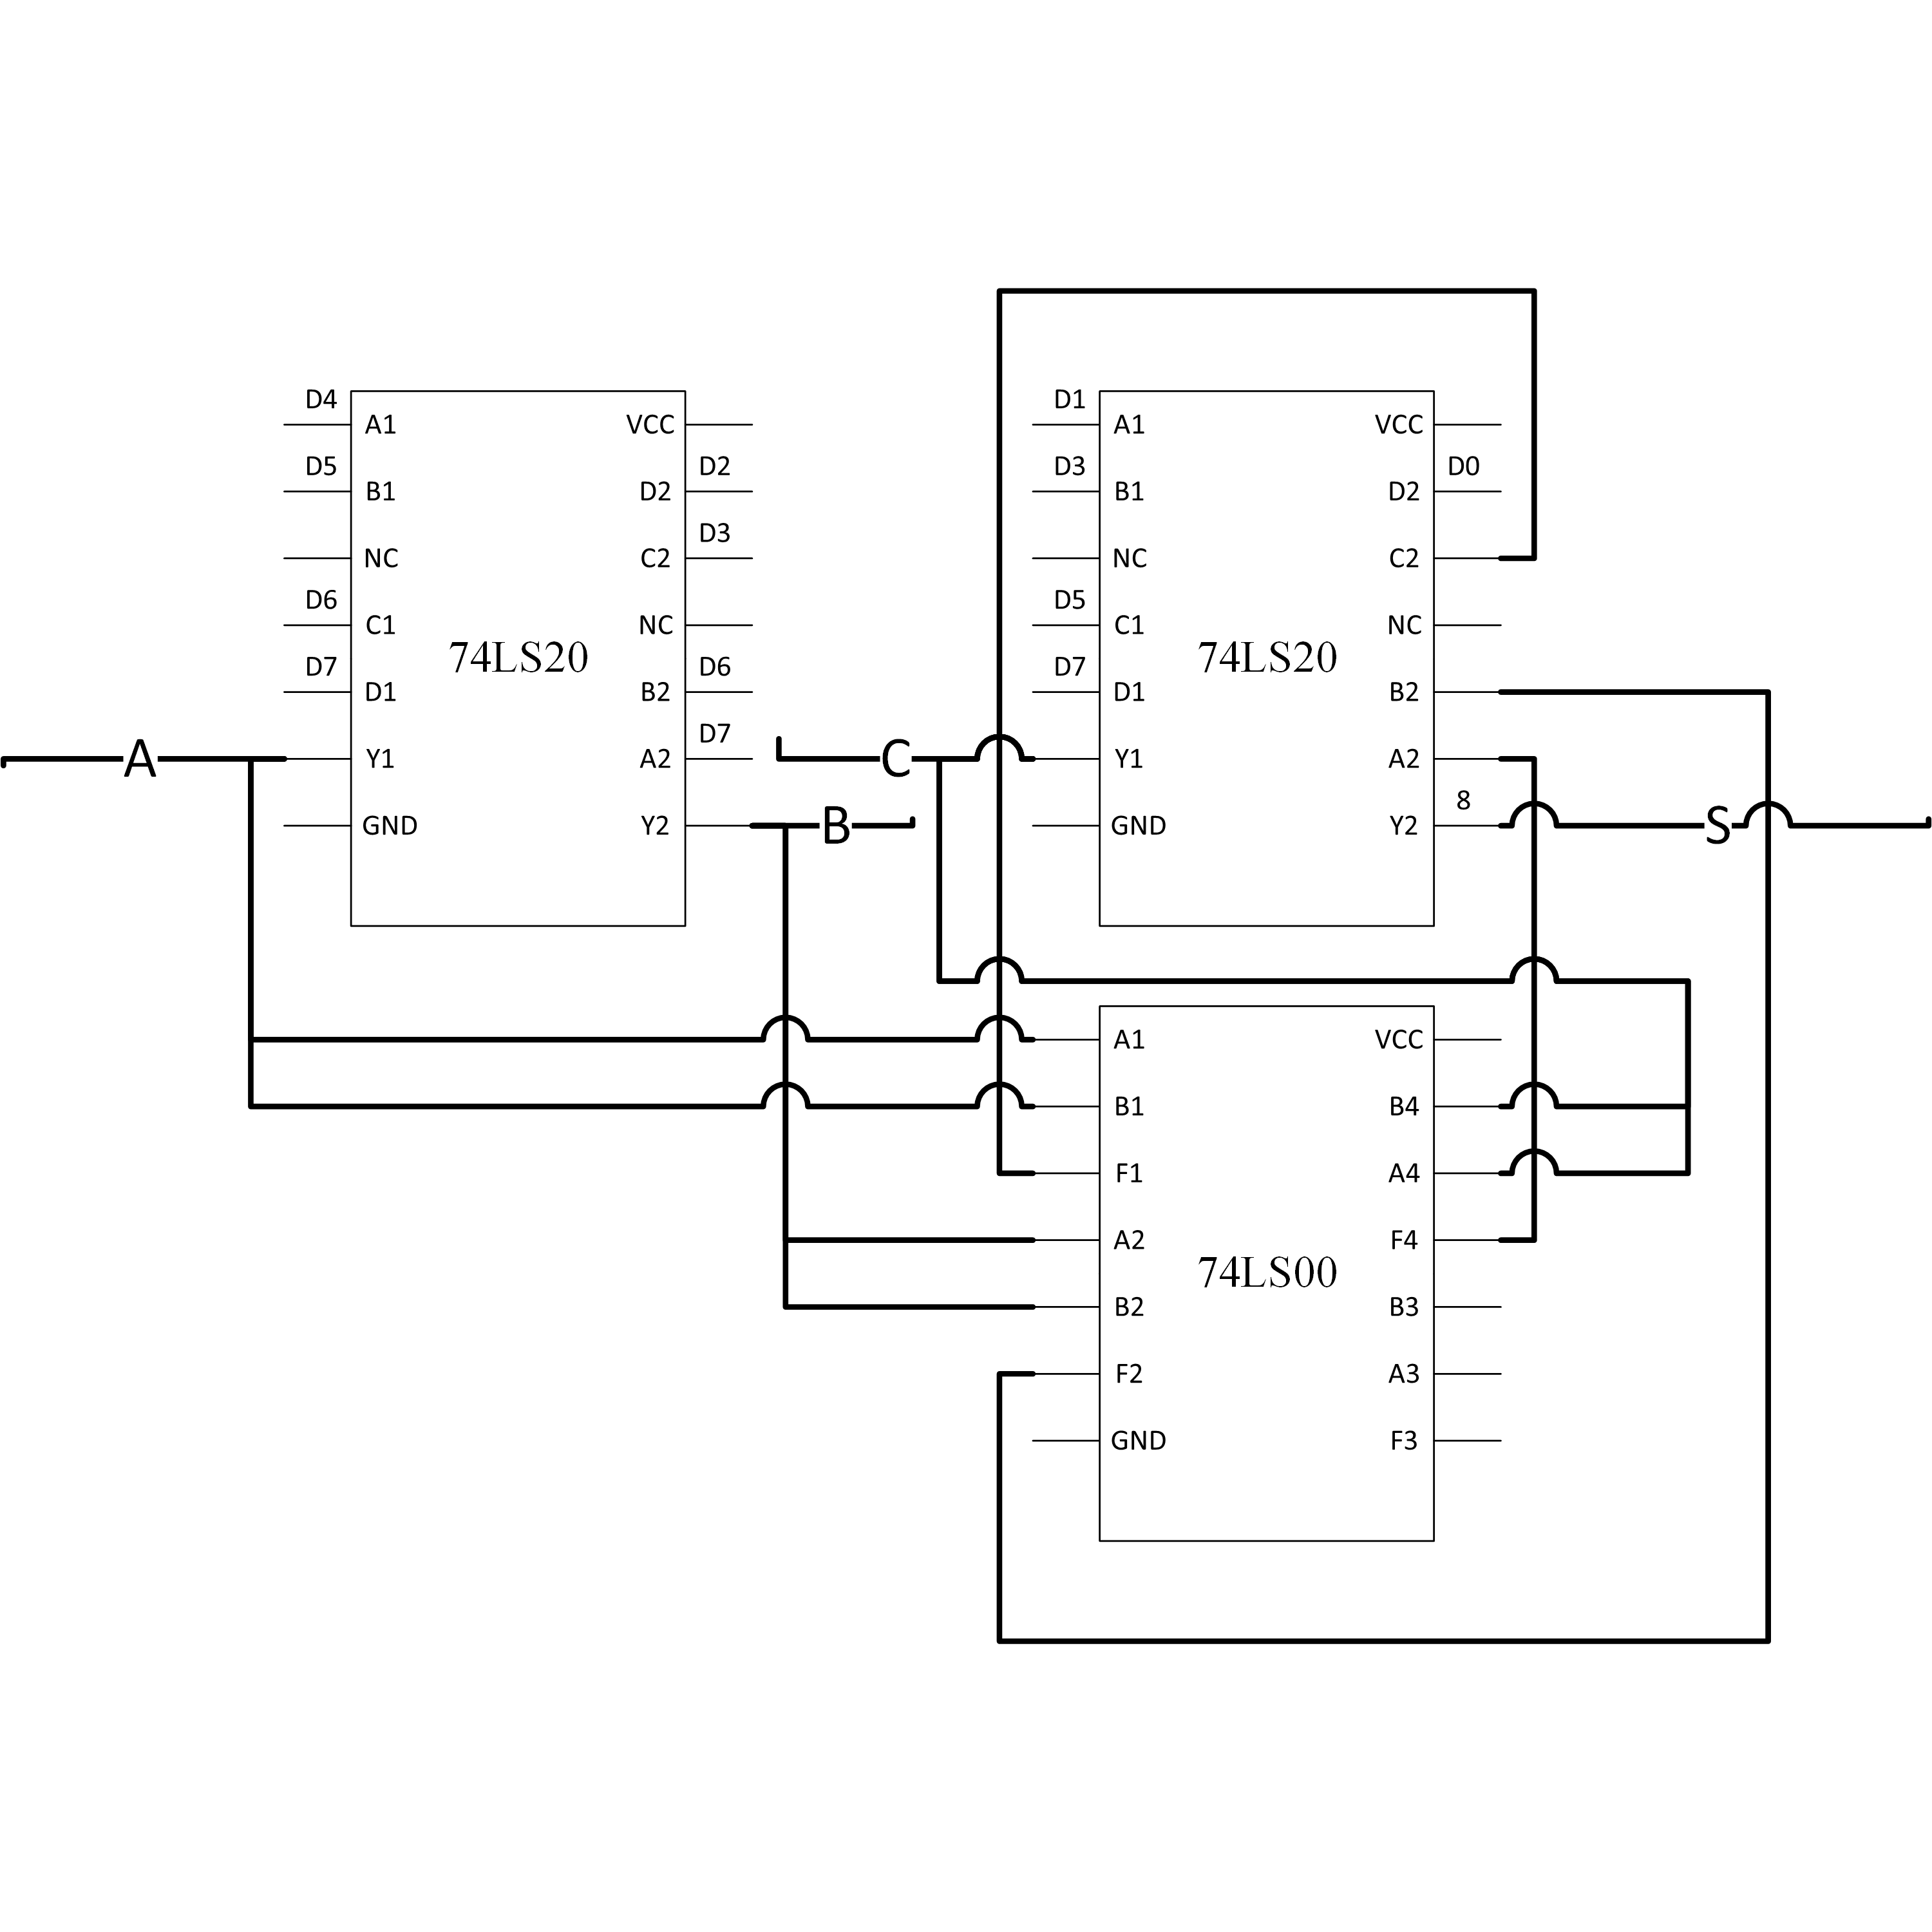
\includegraphics[width=0.6\textwidth]{images/31.png}
\end{figure}

\subsection{2-4译码器}

首先列出2-4进制译码器的真值表如表~\ref{tbl:dec24}。可以写出逻辑表达式\eqref{eqn:dec24}。


\begin{table}[htbp]
	\centering
	\caption{2-4译码器真值表}
	\label{tbl:dec24}
	\begin{tabular}{cc|cccc}
		\toprule
		\hline
		A&B&$Y_0$&$Y_1$&$Y_2$&$Y_3$\\
		\hline
		0&0&0&1&1&1\\
		0&1&1&0&1&1\\
		1&0&1&1&0&1\\
		1&1&1&1&1&0\\
		\hline
		\bottomrule
	\end{tabular}
\end{table}

\begin{equation}
	\label{eqn:dec24}
	\begin{aligned}
		Y_0&=A+B=\ols{\ols{A}\ols{B}}\\
		Y_1&=\ols{A}\ols{B}+\ols{A}B+AB=\ols{A\ols{B}}\\
		Y_2&=\ols{A}\ols{B}+A\ols{B}+AB=\ols{\ols{A}B}\\
		Y_3&=\ols{A}\ols{B}+\ols{A}B+A\ols{B}=\ols{AB}\\
	\end{aligned}
\end{equation}

据此画出电路图如图~\ref{fig:dec24}。

\begin{figure}[H]
	\centering
	\caption{实现2-4译码器}
	\label{fig:dec24}
	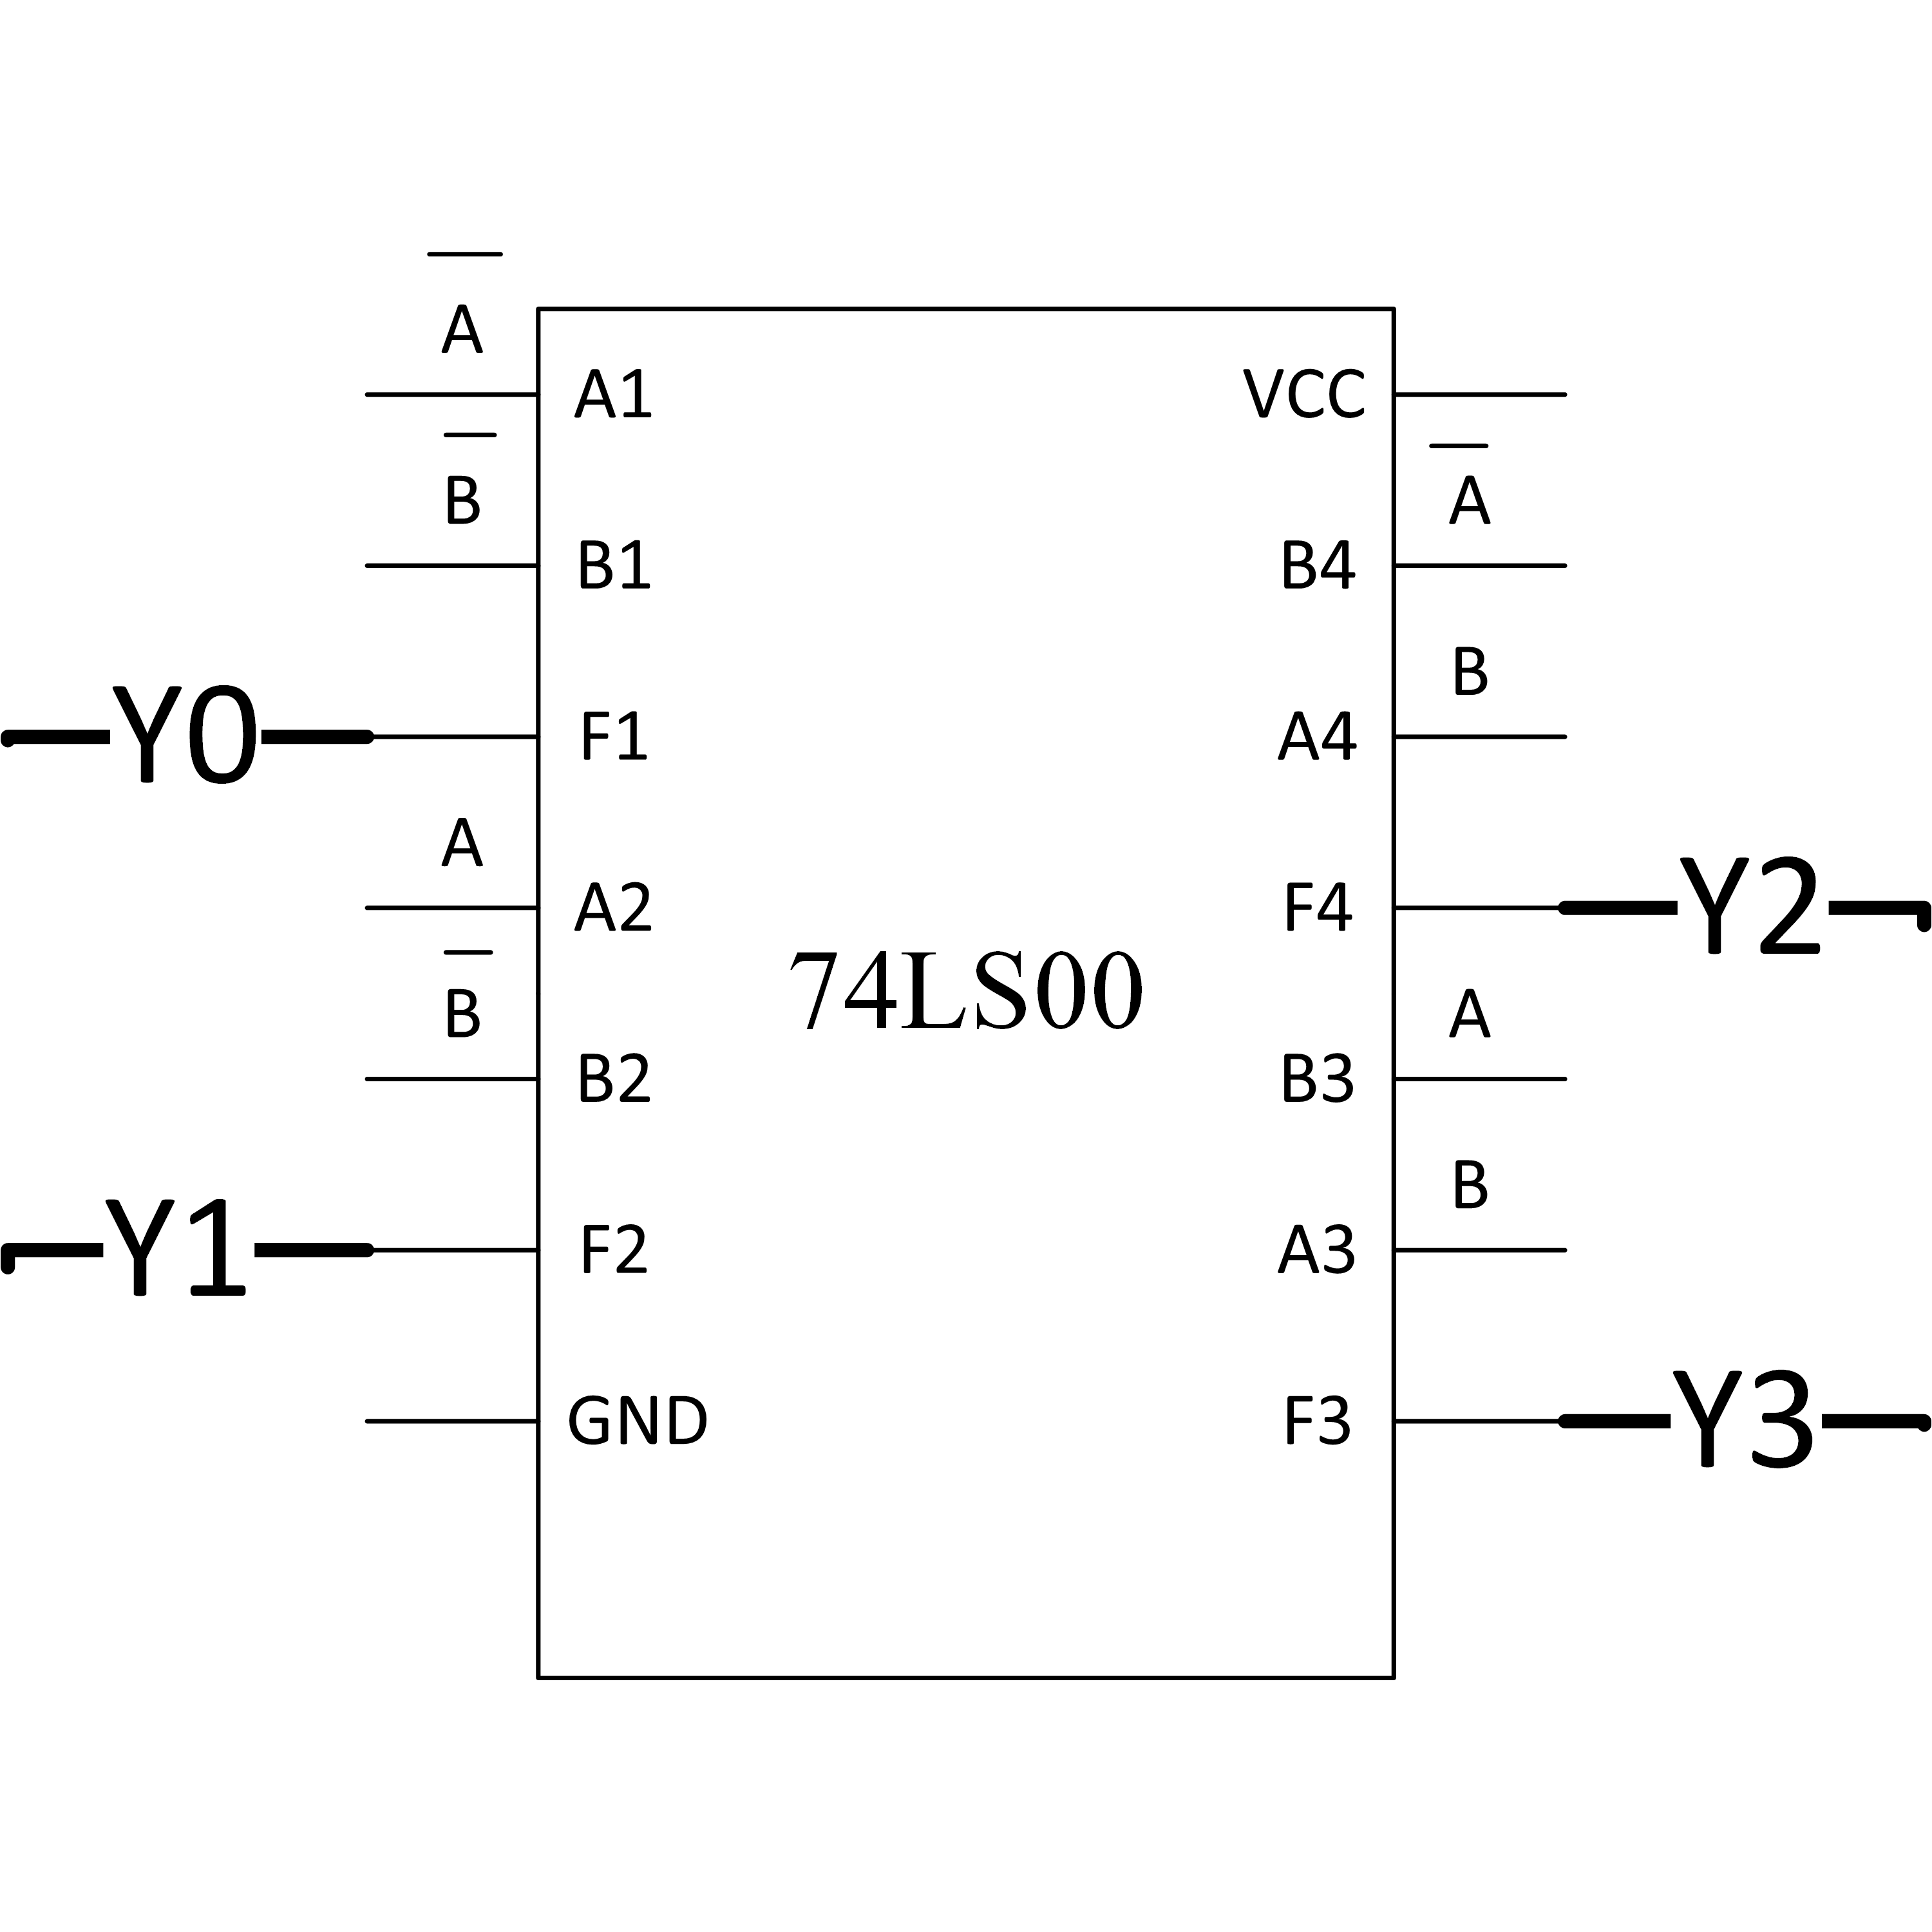
\includegraphics[width=0.32\textwidth]{images/32.png}
\end{figure}

\section{实验结果}

\subsection{2-8进制编码器}

按照图连接电路,得到图

填写真值表,得到表~\ref{tbl:resenc28},可见实验结果是正确的。


\begin{table}[htbp]
	\centering
	\caption{2-8进制编码器真值表}
	\label{tbl:resenc28}
	\begin{tabular}{c|cccccccc|ccc|c}
		\toprule
		\hline 
		十进制数&$D_7$&$D_6$&$D_5$&$D_4$&$D_3$&$D_2$&$D_1$&$D_0$&A&B&C&S \\
		\hline
		0&0&0&0&0&0&0&0&0&0&0&0&0 \\
		0&0&0&0&0&0&0&0&1&0&0&0&1 \\
		1&0&0&0&0&0&0&1&0&0&0&1&1 \\
		2&0&0&0&0&0&1&0&0&0&1&0&1 \\
		3&0&0&0&0&1&0&0&0&0&1&1&1 \\
		4&0&0&0&1&0&0&0&0&1&0&0&1 \\
		5&0&0&1&0&0&0&0&0&1&0&1&1 \\
		6&0&1&0&0&0&0&0&0&1&1&0&1 \\
		7&1&0&0&0&0&0&0&0&1&1&1&1 \\
		\hline
		\bottomrule
	\end{tabular}
\end{table}


\subsection{2-4译码器}

按照图连接电路,得到图

\begin{figure}[htbp]
	\centering
	\caption{实现2-4译码器}
	\label{fig:resdec24}
	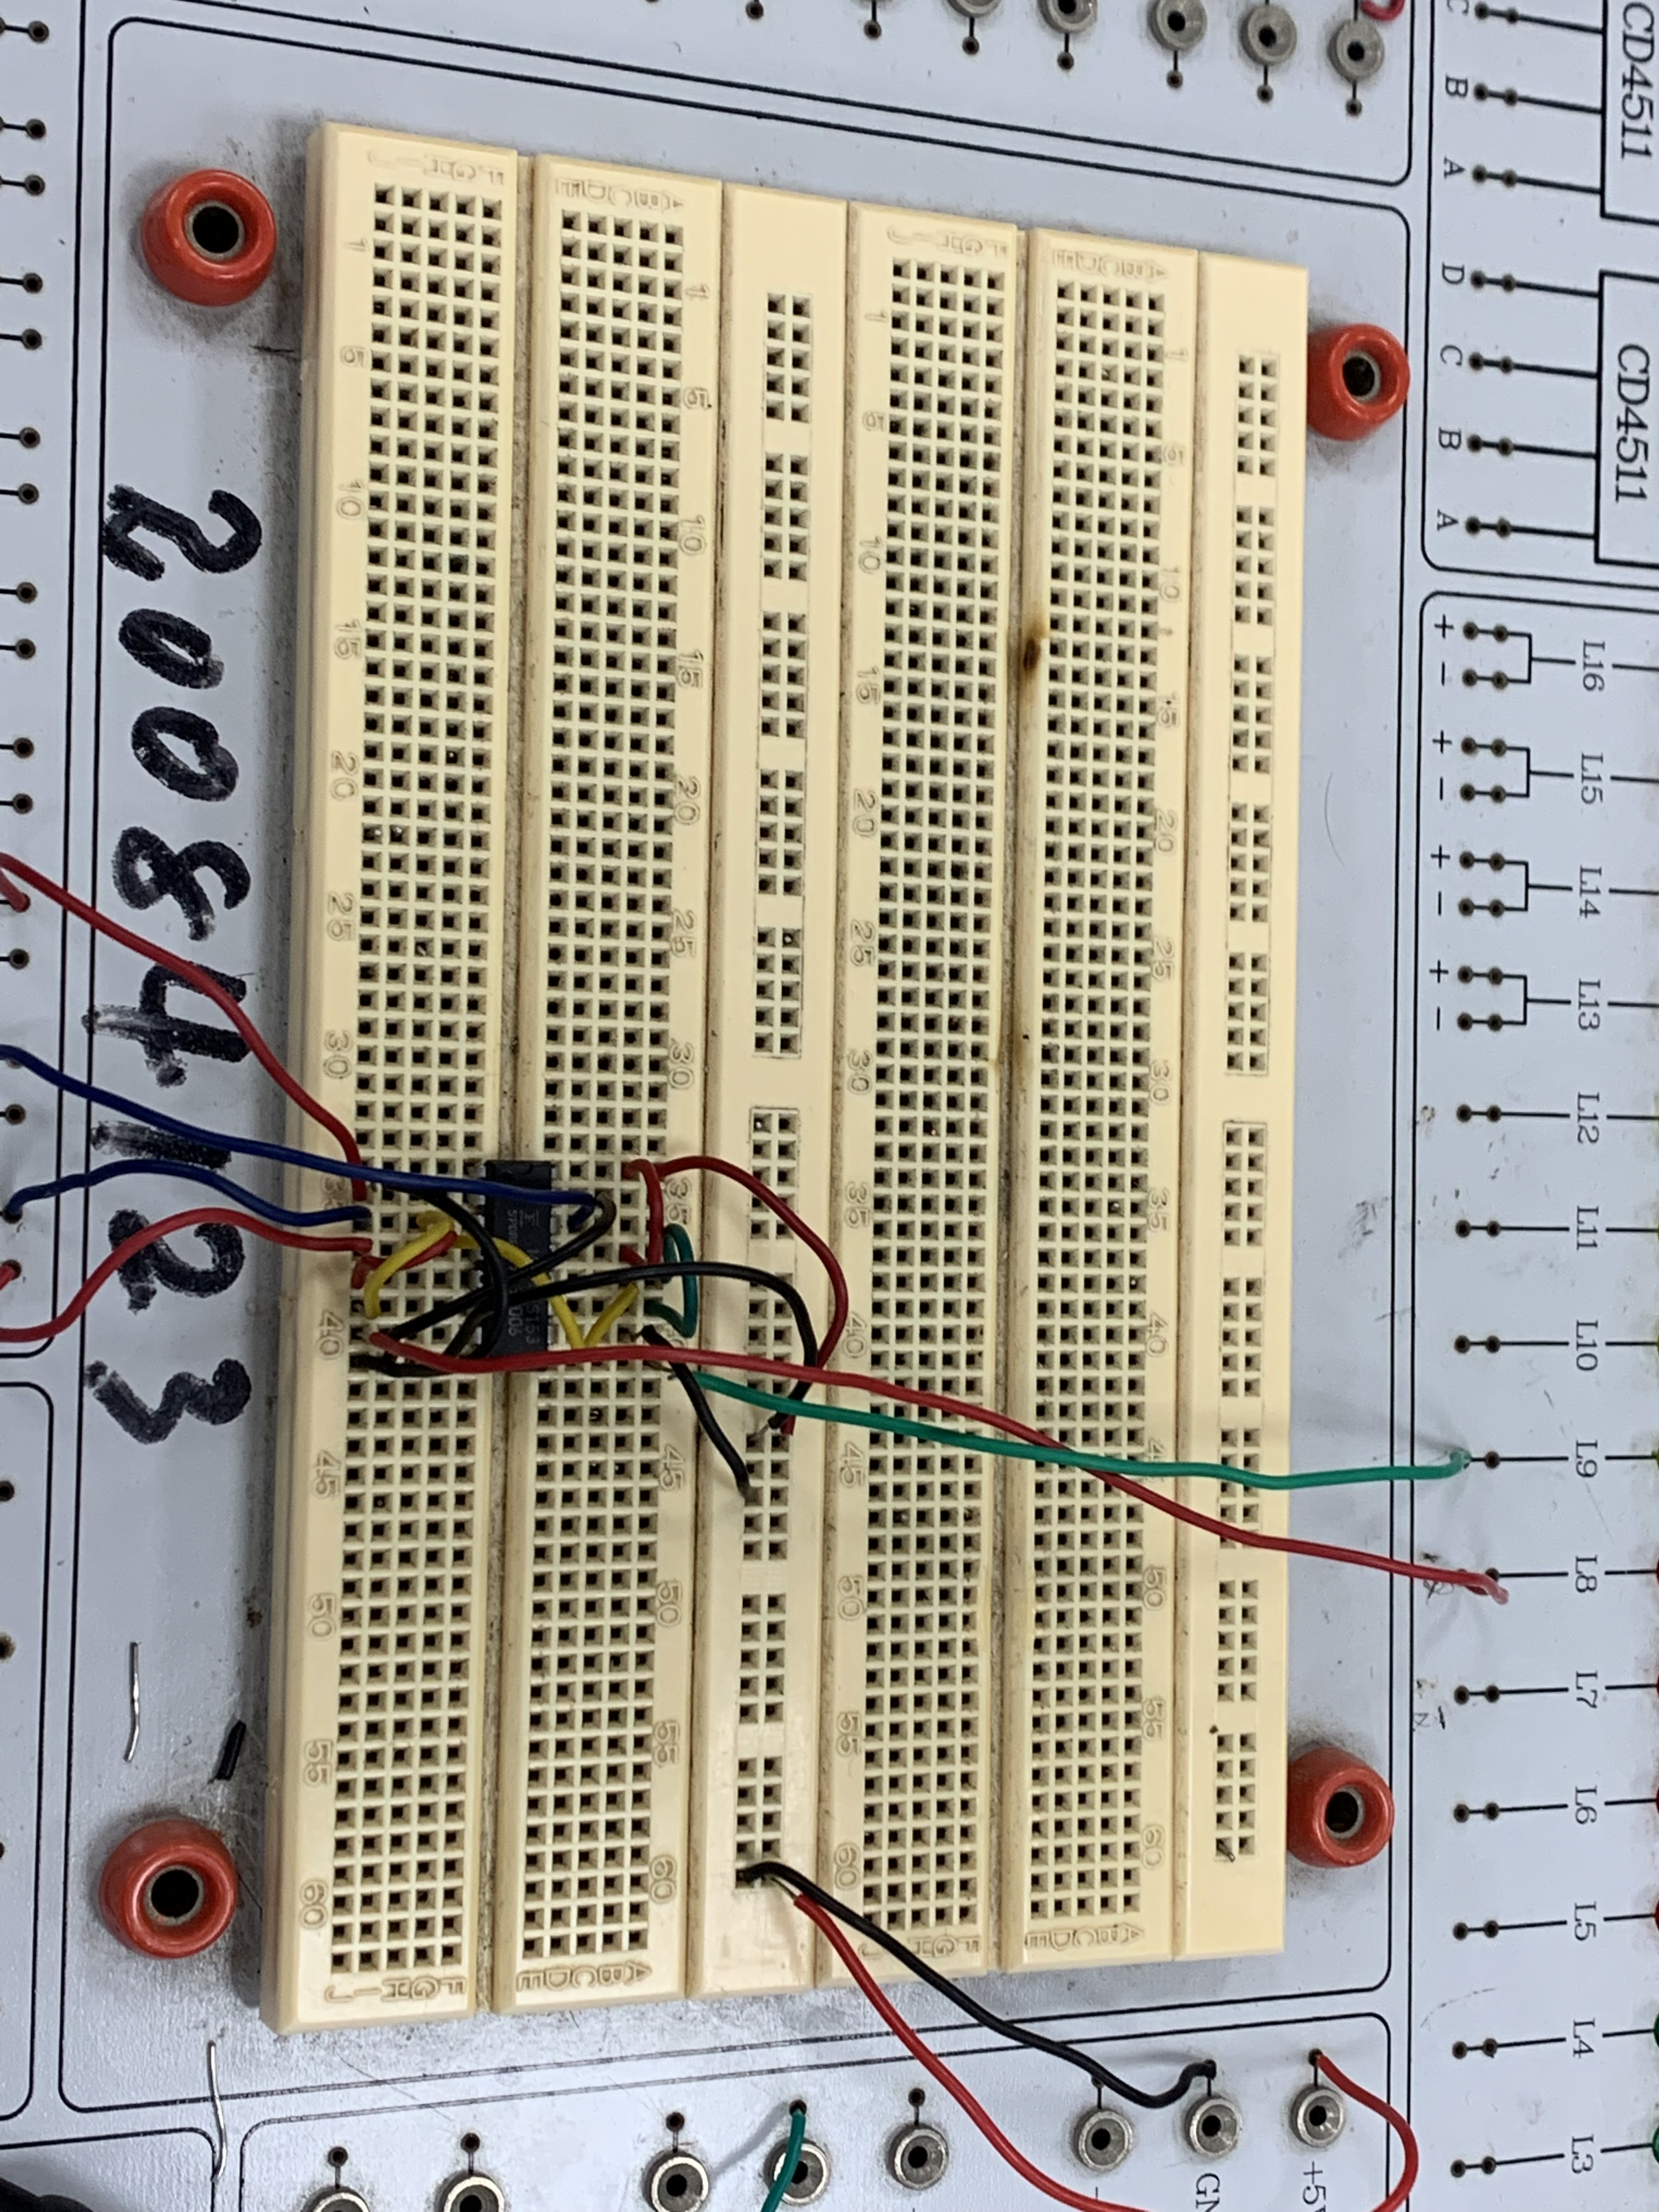
\includegraphics[width=0.42\textwidth,angle=90,origin=c]{images/32.JPG}
\end{figure}

填写真值表,得到表~\ref{tbl:resdec24},可见实验结果是正确的。

\begin{table}[htbp]
	\centering
	\caption{2-4译码器真值表}
	\label{tbl:resdec24}
	\begin{tabular}{cc|cccc}
		\toprule
		\hline
		A&B&$Y_0$&$Y_1$&$Y_2$&$Y_3$\\
		\hline
		0&0&0&1&1&1\\
		0&1&1&0&1&1\\
		1&0&1&1&0&1\\
		1&1&1&1&1&0\\
		\hline
		\bottomrule
	\end{tabular}
\end{table}

\section{思考题}

\begin{enumerate}
	\item 有八根地址线(A7、A6、A5、A4、A3、A2、A1、A0),试用 74LS138 及门电路设计一个
	地址译码电路,当输入地址为 30H 时,输出 Y0 为 0,当输入地址为 31H 时,输出 Y1 为 0。	
\end{enumerate}

已知$30H$和$31H$的二进制表示为\eqref{eqn:bin3031}

\begin{equation}
	\label{eqn:bin3031}
	\begin{aligned}
		30H&=0011,0000B\\
		31H&=0011,0001B
	\end{aligned}
\end{equation}

因此可以列出74LS138的使能端和输入端的真值表,如表\ref{tbl:dec}

\begin{table}[htbp]
	\centering
	\caption{真值表}
	\label{tbl:dec}
	\begin{tabular}{cccccccc|cccc}
		\toprule
		\hline
		A7&A6&A5&A4&A3&A2&A1&A0&$S_1$&T2&T1&T0\\
		\hline
		0&0&1&1&0&0&0&0&1&0&0&0\\
		0&0&1&1&0&0&0&1&1&0&0&1\\
		0&0&1&1&0&0&0&0&1&0&1&0\\
		0&0&1&1&0&0&0&1&1&0&1&1\\
		0&0&1&1&0&0&0&0&1&1&0&0\\
		0&0&1&1&0&0&0&1&1&1&0&1\\
		0&0&1&1&0&0&0&0&1&1&1&0\\
		0&0&1&1&0&0&0&1&1&1&1&1\\
		$\times$&$\times$&$\times$&$\times$&$\times$&$\times$&$\times$&$\times$&0&0&0&0\\
		\hline
		\bottomrule
	\end{tabular}
\end{table}

根据真值表设计电路如图~\ref{fig:addrdec}

\begin{figure}[H]
	\centering
	\caption{地址译码电路}
	\label{fig:addrdec}
	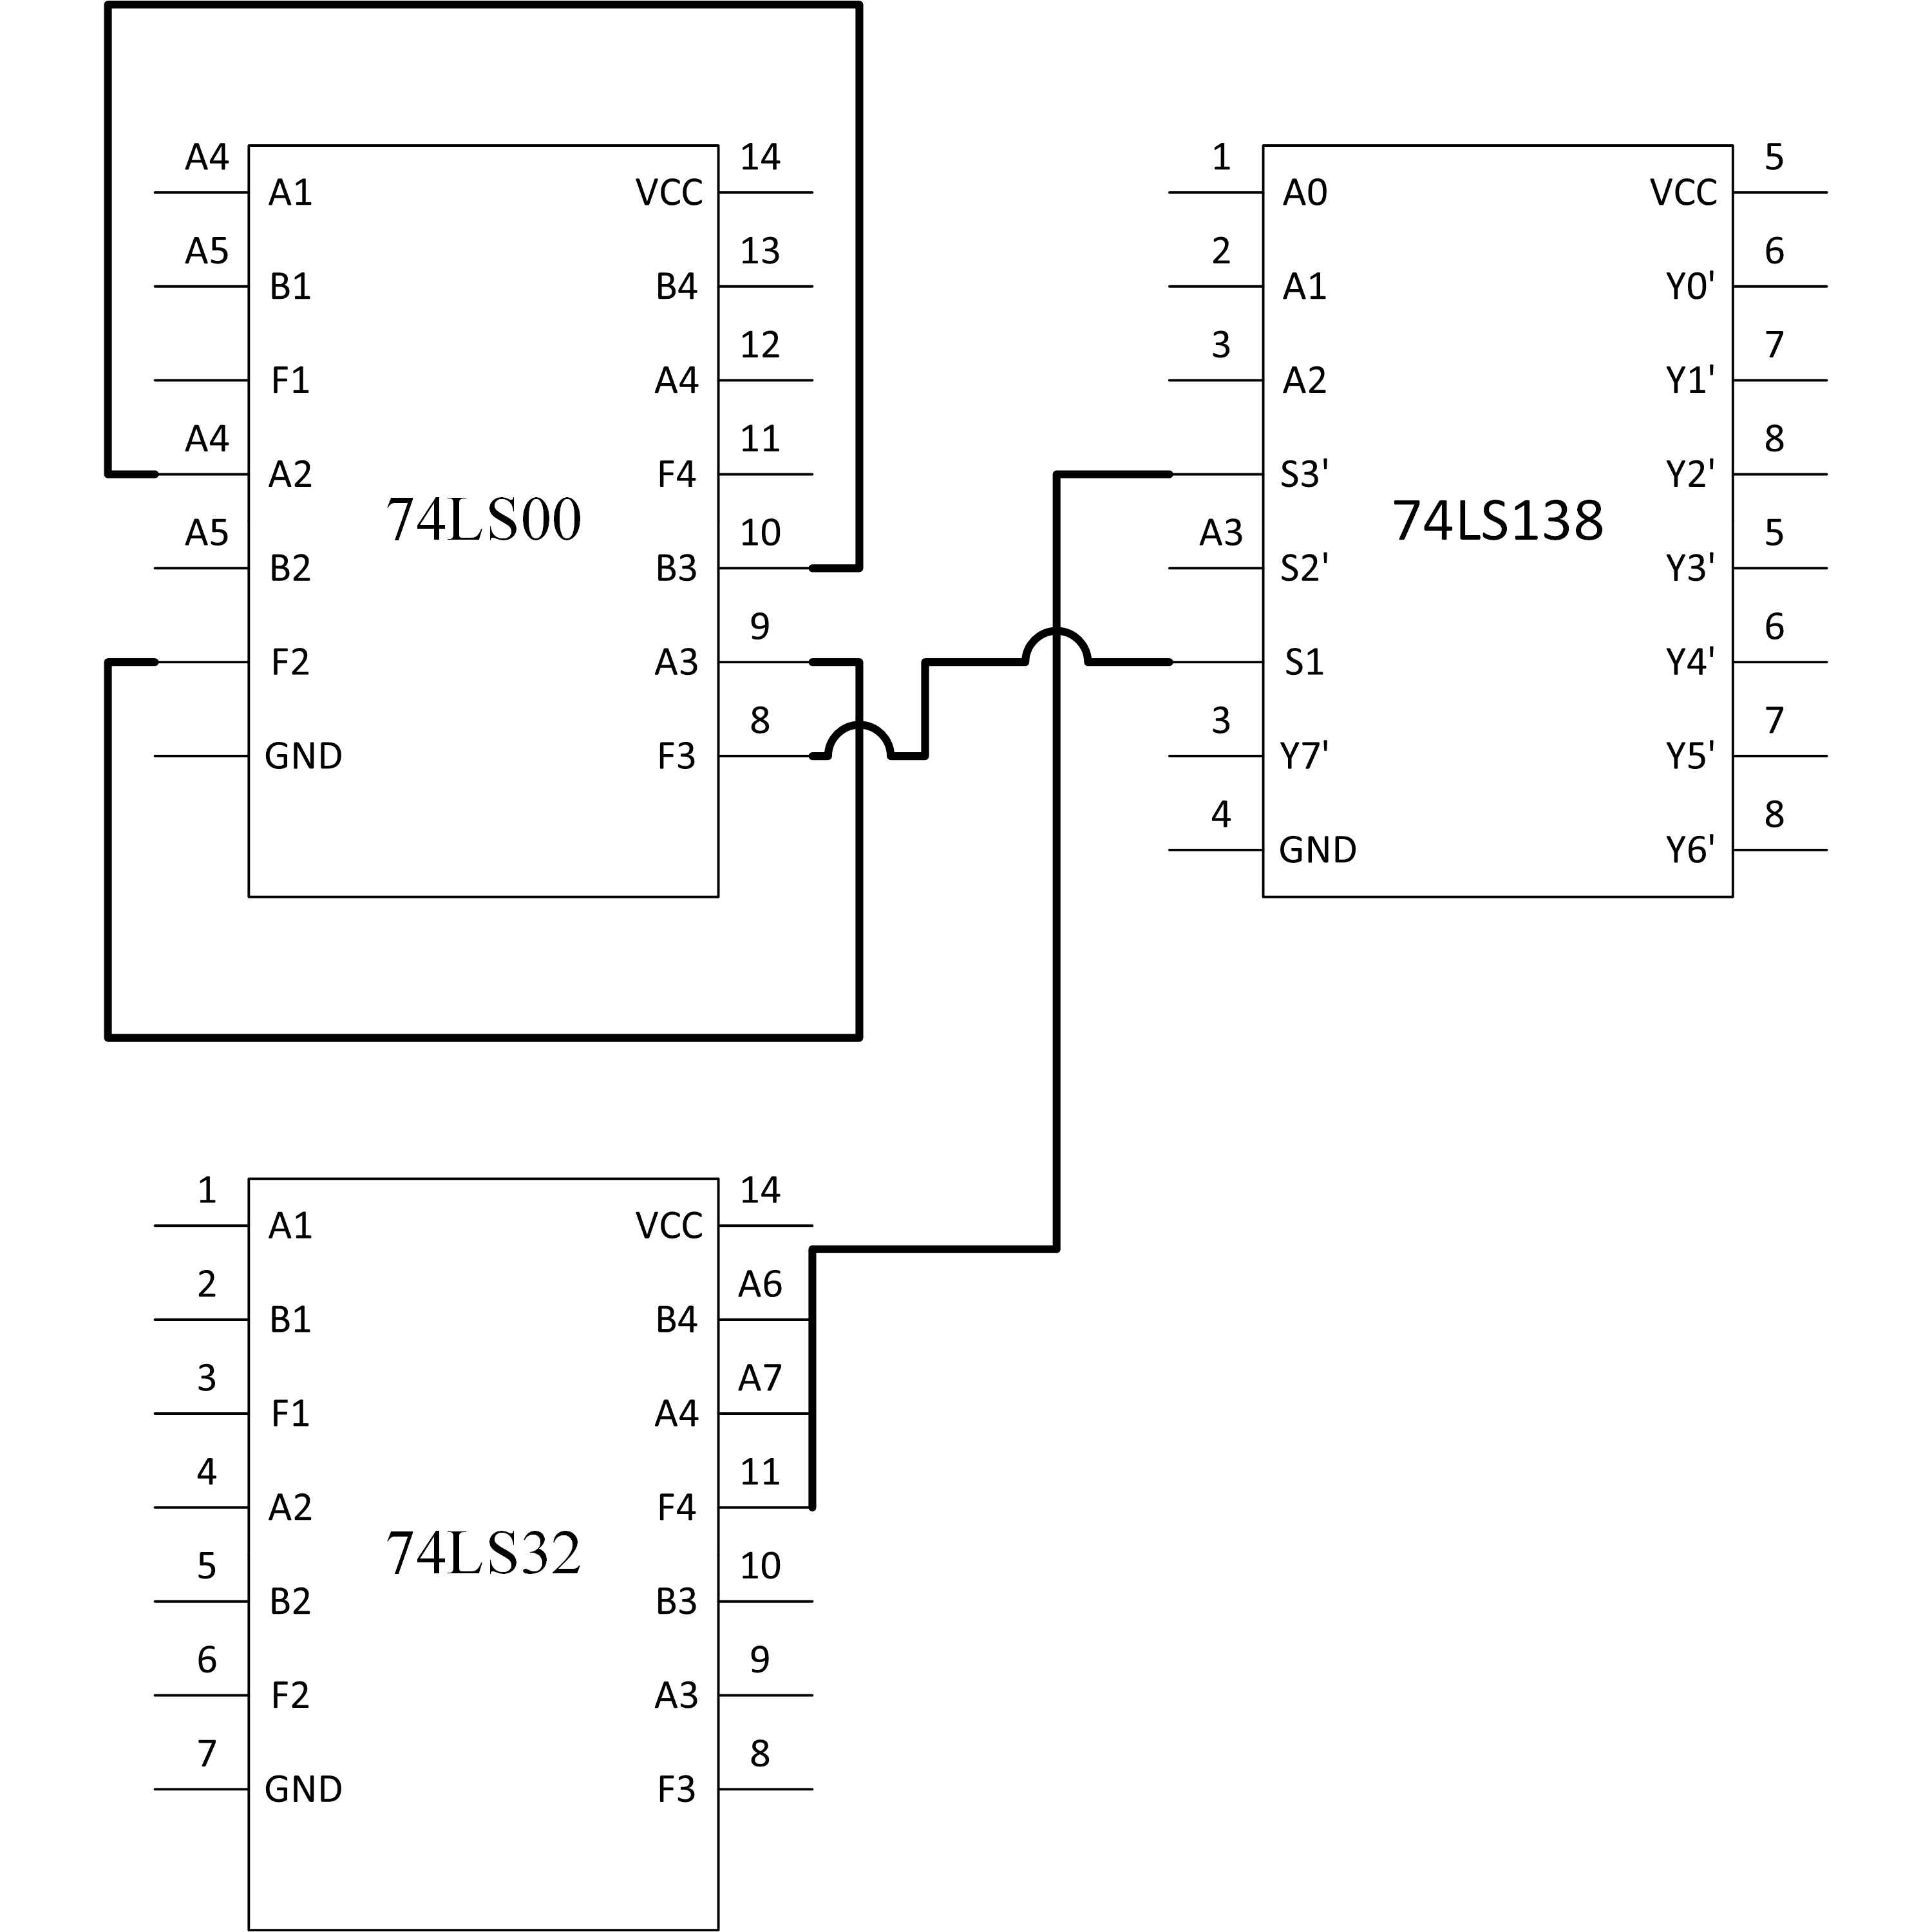
\includegraphics[width=0.32\textwidth]{images/33.png}
\end{figure}

\clearpage


\includepdf[pages={10}]{../instruction.pdf}
\setcounter{section}{4}

\section{电路设计}

\subsection{双2-4译码器构成3-8译码器}

设输入为$G$, $A_1$, $A_2$, $A_3$, 则

\begin{equation}
	\begin{aligned}
		1G=\ols{\ols{G}\ols{A_3}}\\
		1A=A_1\\
		1B=A_2\\
		2G=\ols{\ols{G}A_3}\\
		2A=A_1\\
		2B=A_2\\
	\end{aligned}
\end{equation}

因此可以画出电路图如图~\ref{fig:dec24to38}

\begin{figure}[htbp]
	\centering
	\caption{2-4译码器实现3-8译码器}
	\label{fig:dec24to38}
	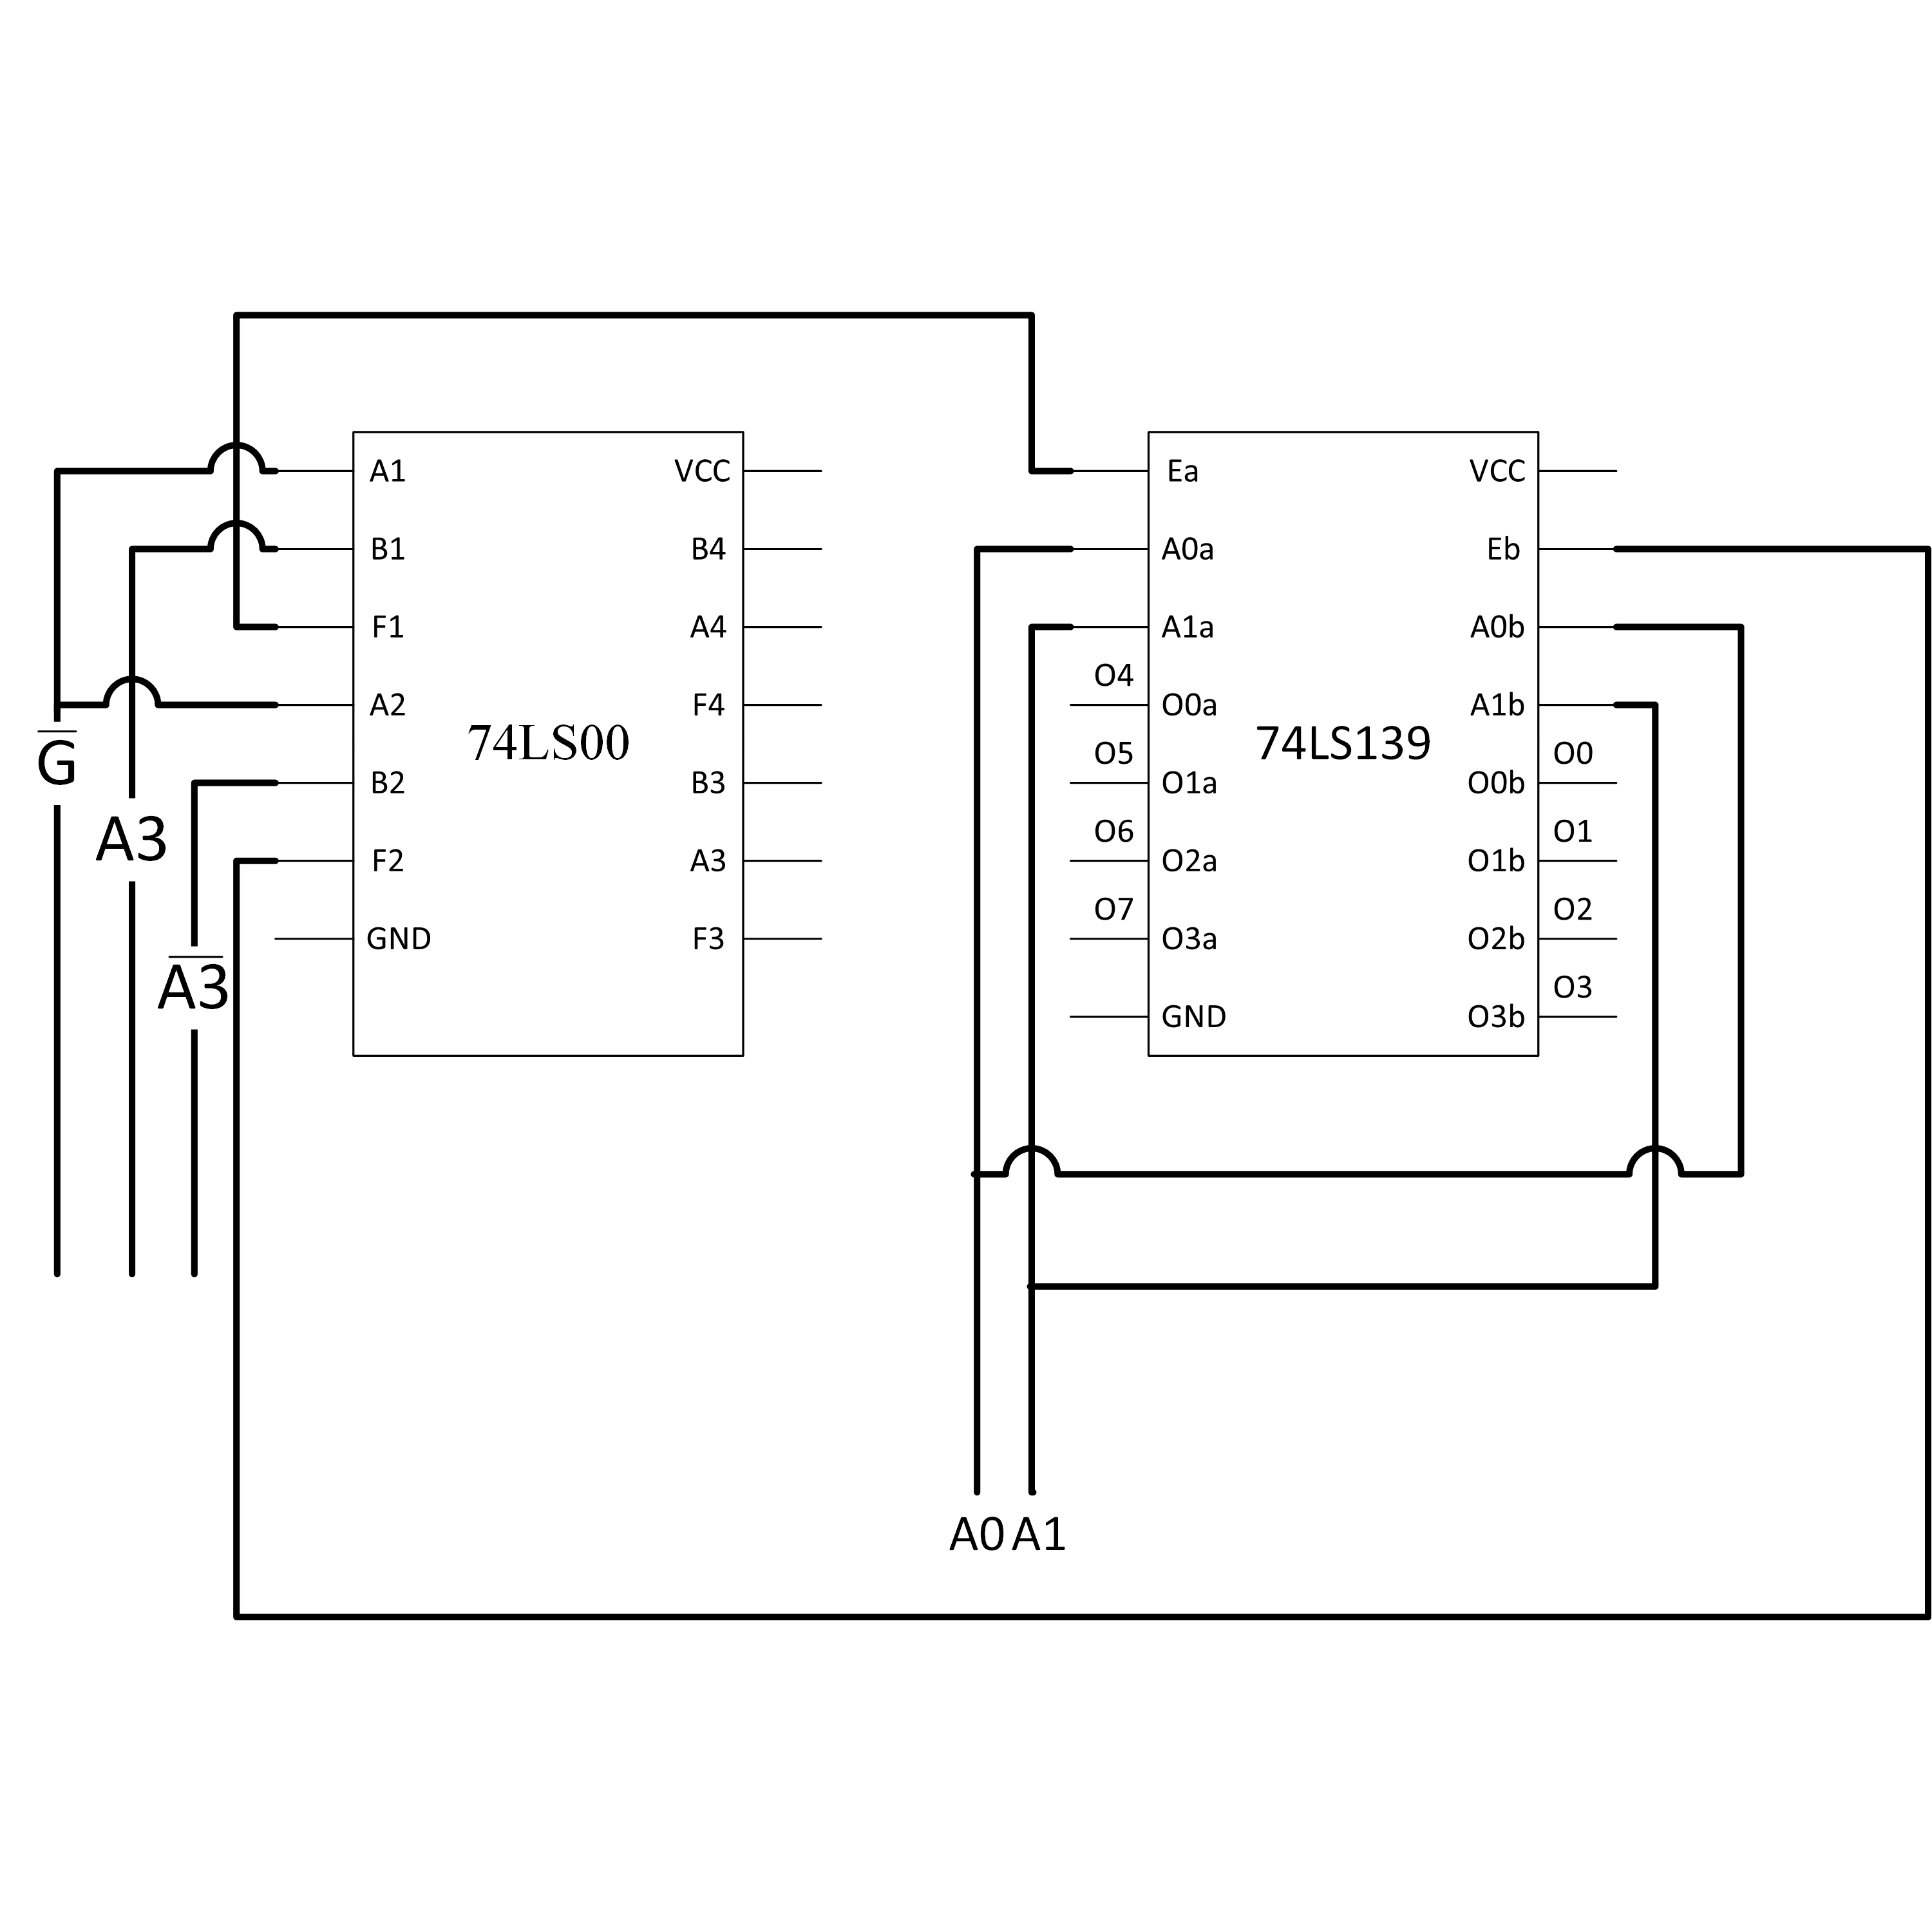
\includegraphics[width=0.48\textwidth]{images/41.png}
\end{figure}

\subsection{用74LS138及与非门实现全加器}

全加器的真值表为表~\ref{tbl:fulladder}。使用3-8译码器实现全加器,需要将逻辑表达式
写成最小项的和。

\begin{table}[htbp]
	\centering
	\caption{全加器}
	\label{tbl:fulladder}
	\begin{tabular}{ccc|cc}
		\toprule
		\hline
		$A_i$&$B_i$&$C_{i-1}$&$S_i$&$C_i$\\
		\hline
		0&0&0&0&0\\
		0&0&1&1&0\\
		0&1&0&1&0\\
		0&1&1&0&1\\
		1&0&0&1&0\\
		1&0&1&0&1\\
		1&1&0&0&1\\
		1&1&1&1&1\\
		\hline
		\bottomrule
	\end{tabular}
\end{table}

因此最小项表达式和化简如\eqref{eqn:fulladderwithdec}

\begin{equation}
	\label{eqn:fulladderwithdec}
	\begin{aligned}
		S_i&=m_1+m_2+m_4+m_7\\
		&=\ols{\ols{m_1}\ols{m_2}\ols{m_4}\ols{m_7}}\\
		C_i&=m_3+m_5+m_6+m_7\\
		&=\ols{\ols{m_3}\ols{m_5}\ols{m_6}\ols{m_7}}\\
	\end{aligned}
\end{equation}

因此可以画出电路图如图~\ref{fig:fulladder138}

\begin{figure}[htbp]
	\centering
	\caption{用74LS138及与非门实现全加器}
	\label{fig:fulladder138}
	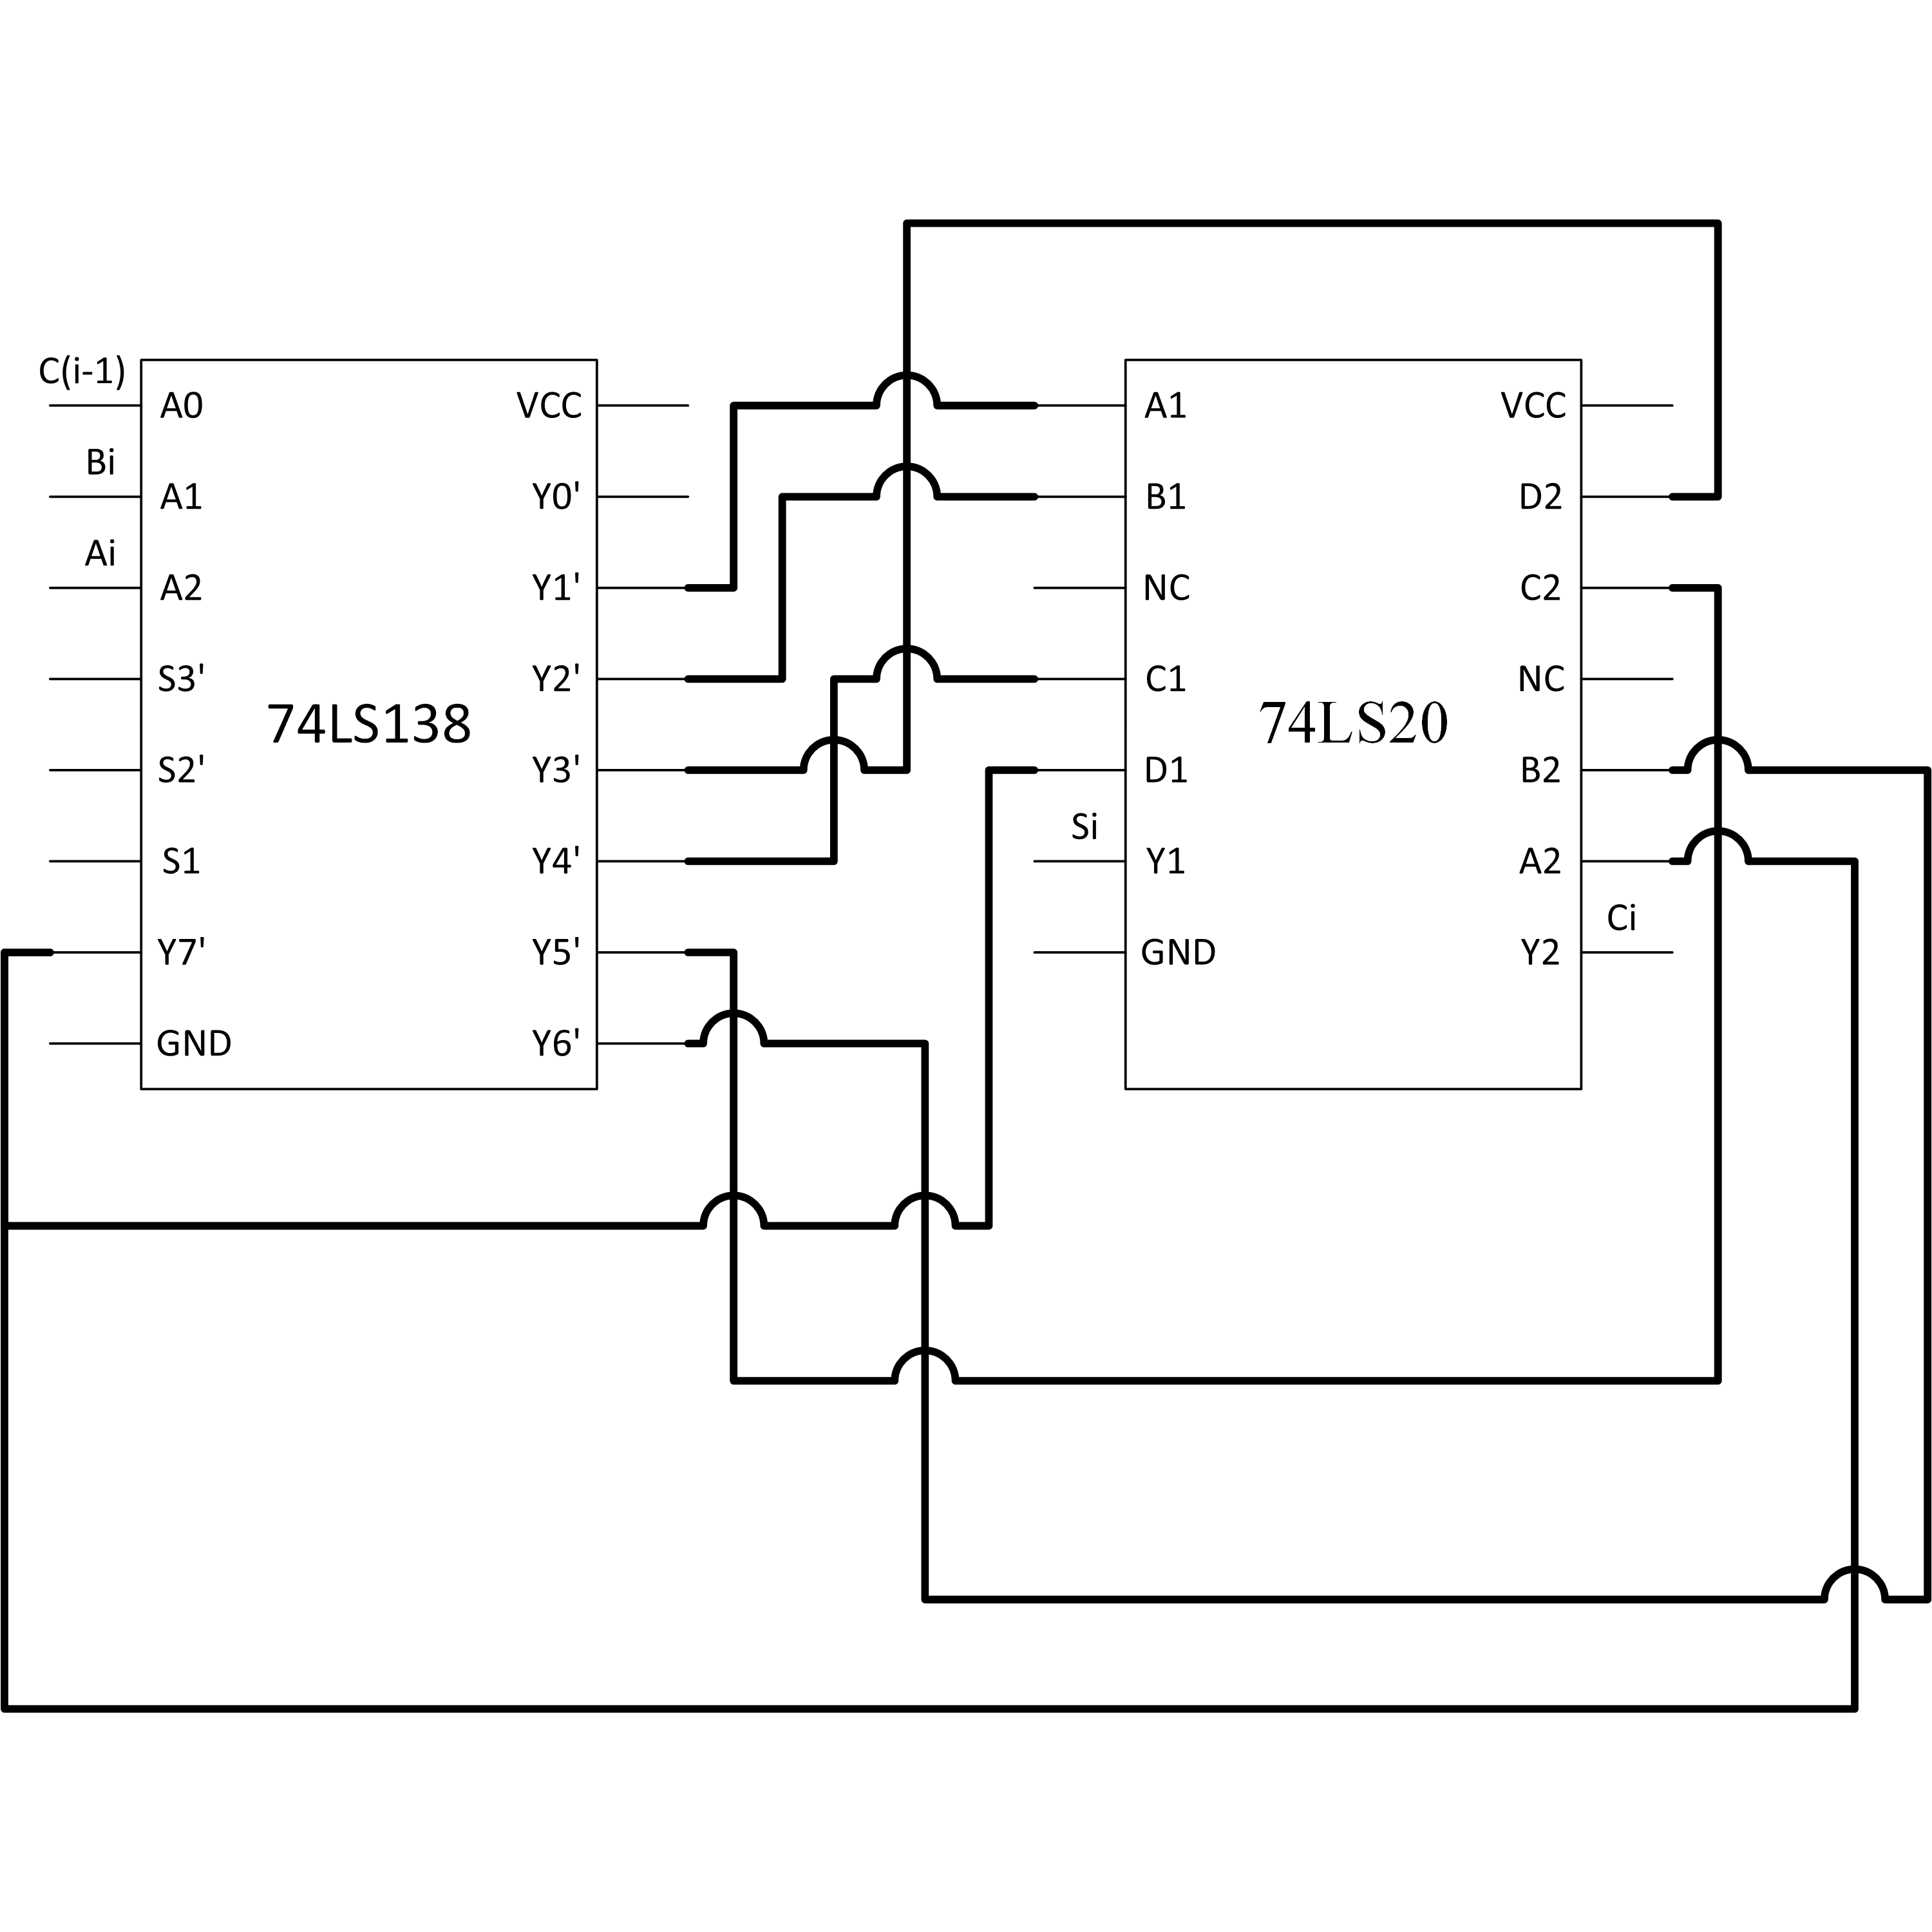
\includegraphics[width=0.48\textwidth]{images/42.png}
\end{figure}

\subsection{用74LS153及与非门实现全加器}

用4选1多路选择器实现全加器,需要选择地址选择变量,需要使用卡诺图,如图~\ref{eqn:knm}。
选择$A_i B_i$为地址选择端。

\begin{figure}[htbp]
	\centering
	\caption{$S_i$和$C_i$的卡诺图}
	\label{eqn:knm}
	\subfigure{
		\begin{karnaugh-map}(label=corner)[4][2][1][$C_{i-1}$][$B_i$][$A_i$]
			\minterms{1,2,3,4,7}
			\implicant{0}{4}
			\implicant{1}{5}
			\implicant{2}{6}
			\implicant{3}{7}
		\end{karnaugh-map}
	}
	~
	\subfigure{
		\begin{karnaugh-map}(label=corner)[4][2][1][$C_{i-1}$][$B_i$][$A_i$]
			\minterms{5,6,7}
			\implicant{0}{4}
			\implicant{1}{5}
			\implicant{2}{6}
			\implicant{3}{7}
		\end{karnaugh-map}
	}
\end{figure}

根据卡诺图,可以将表达式写为\eqref{eqn:fulladderwithmux}

\begin{equation}
	\label{eqn:fulladderwithmux}
	\begin{aligned}
		S_i&=\ols{A_i}\ols{B_i} \cdot C_{i-1}+ A_i\ols{B_i}\cdot \ols{C_{i-1}}+ \ols{A_i}B_i\cdot 1+A_iB_i\cdot \ols{C_{i-1}}\\
		C_i&=\ols{A_i}\ols{B_i} \cdot 0+ A_i\ols{B_i}\cdot C_{i-1}+ \ols{A_i}B_i\cdot 0+A_iB_i\cdot 1\\
	\end{aligned}
\end{equation}

因此可以画出电路图如图~\ref{fig:fulladder153}

\begin{figure}[htbp]
	\centering
	\caption{用74LS153及与非门实现全加器}
	\label{fig:fulladder153}
	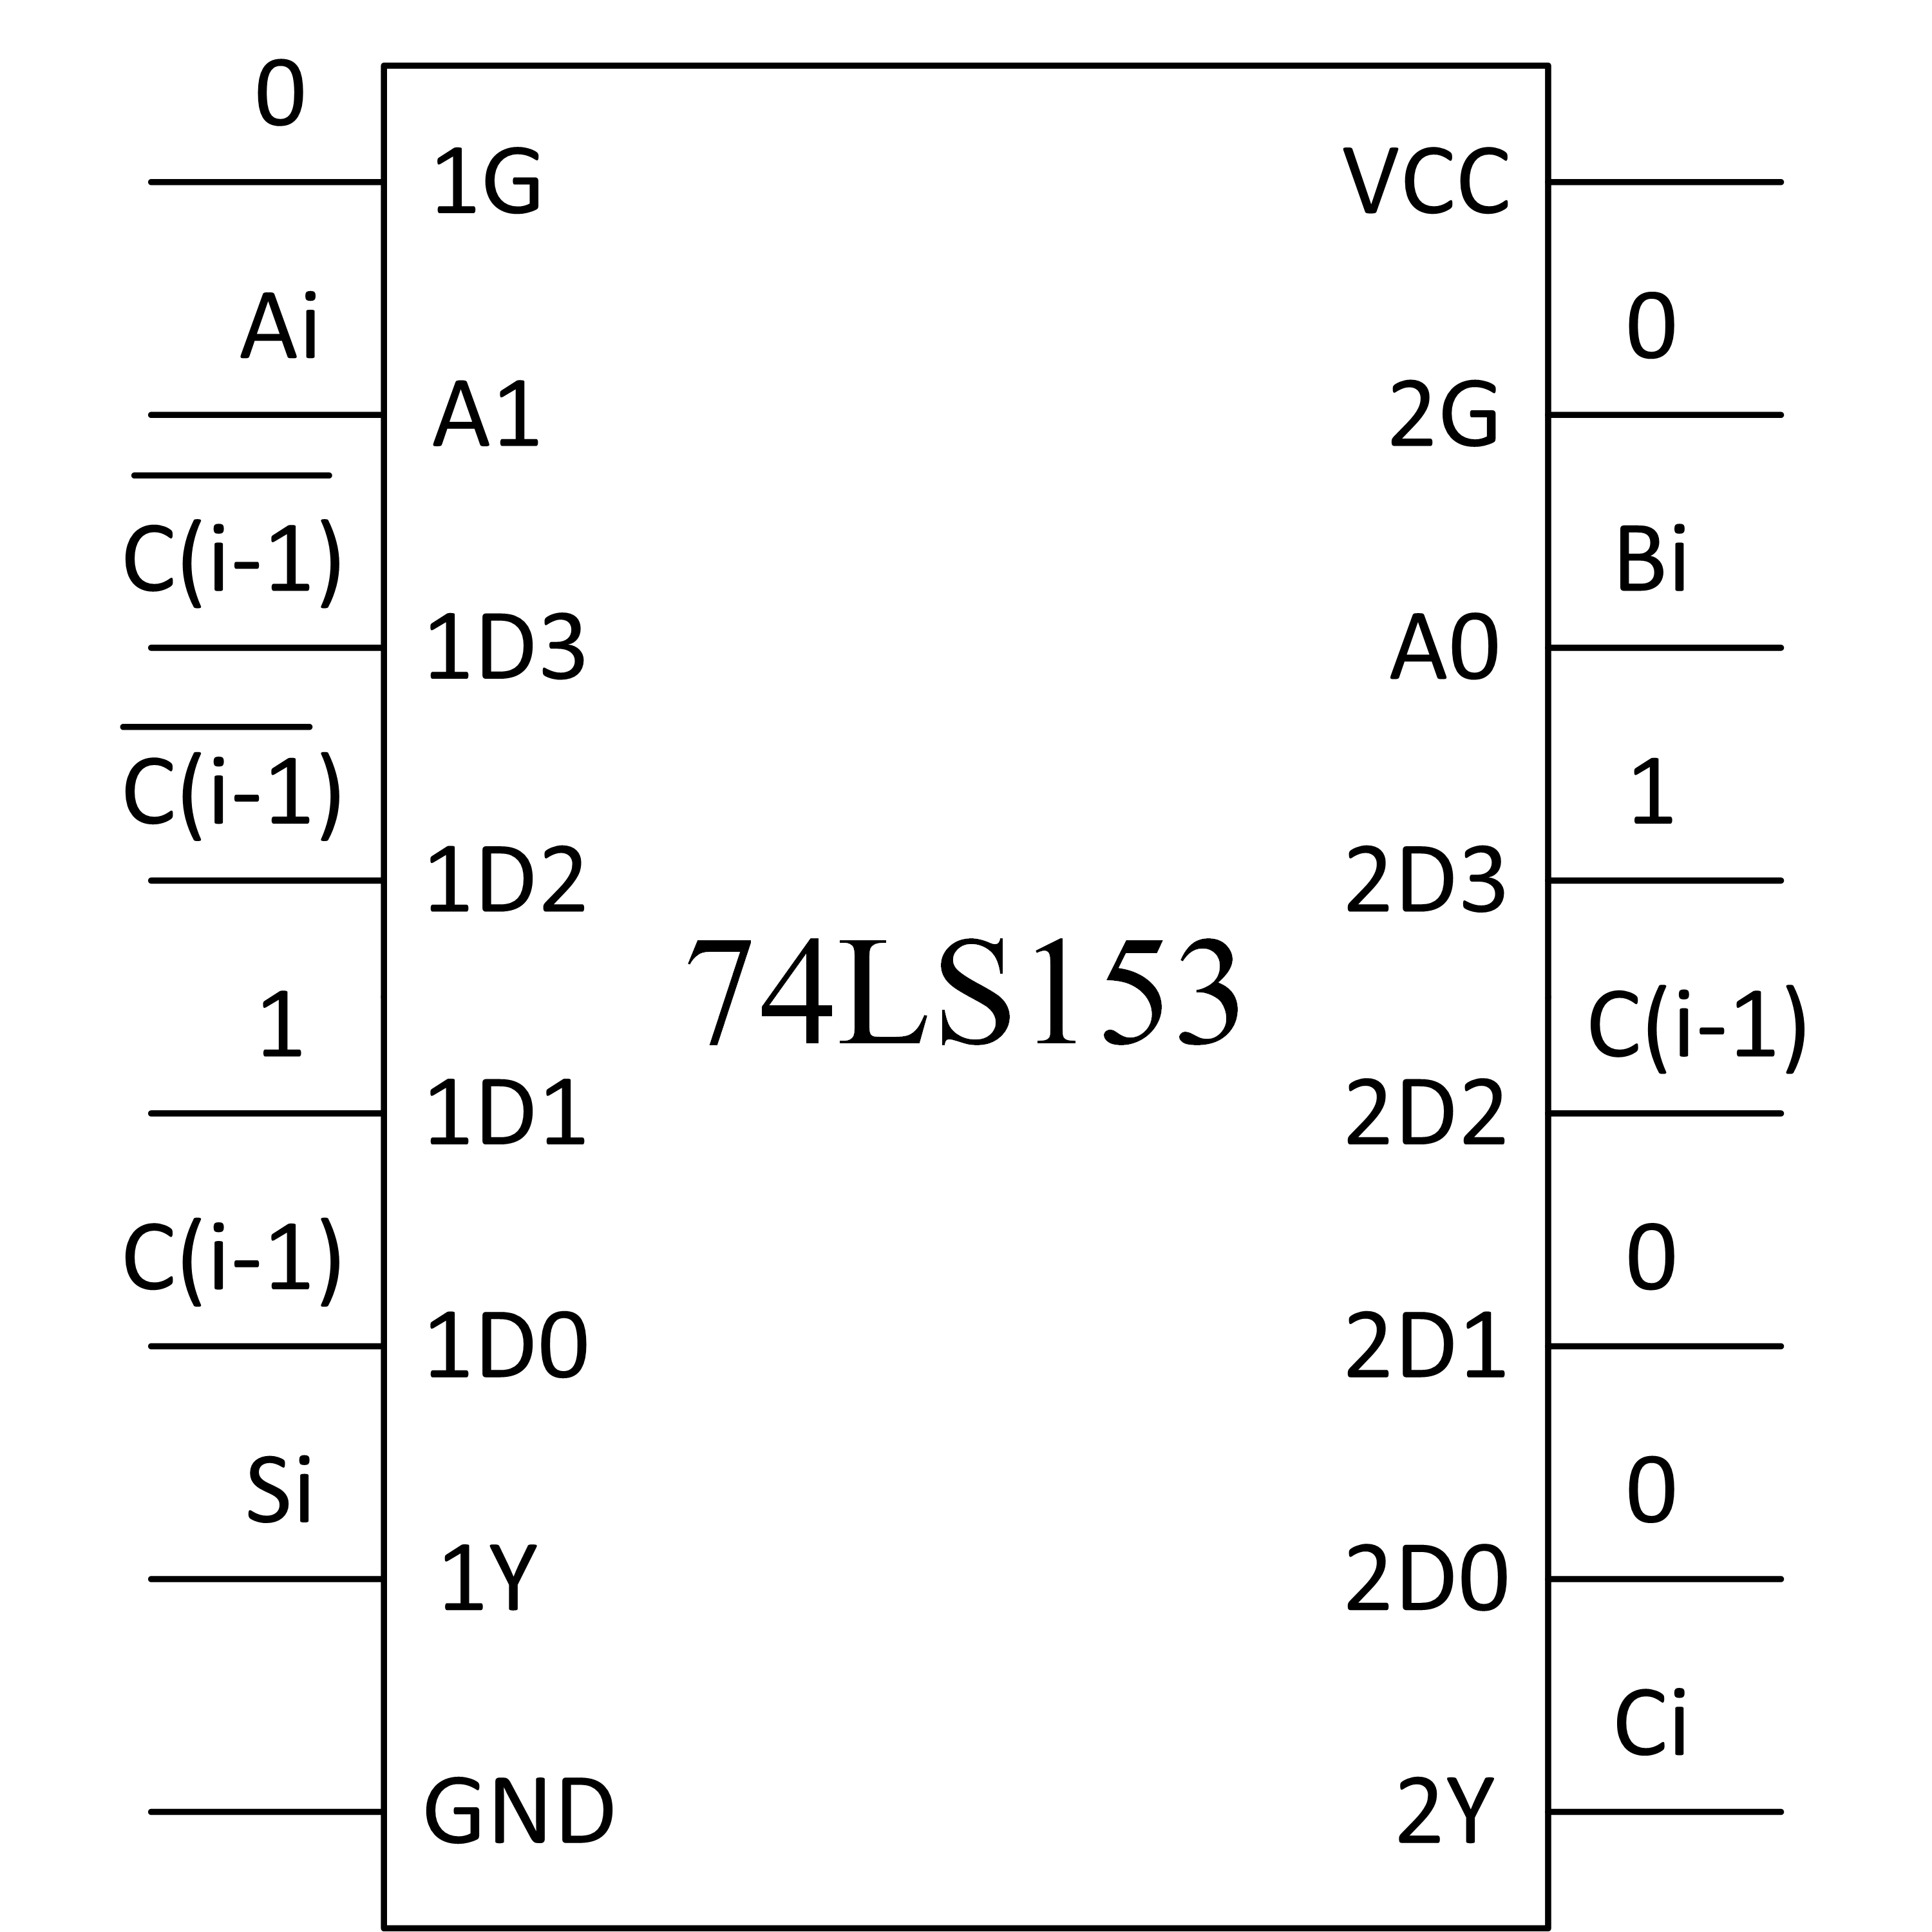
\includegraphics[width=0.32\textwidth]{images/43.png}
\end{figure}

\section{实验结果}

\subsection{3-8译码器实现全加器}

按照图连接电路,得到图~\ref{fig:resfulladder153}

\begin{figure}[htbp]
	\centering
	\caption{用74LS153及与非门实现全加器}
	\label{fig:resfulladder153}
	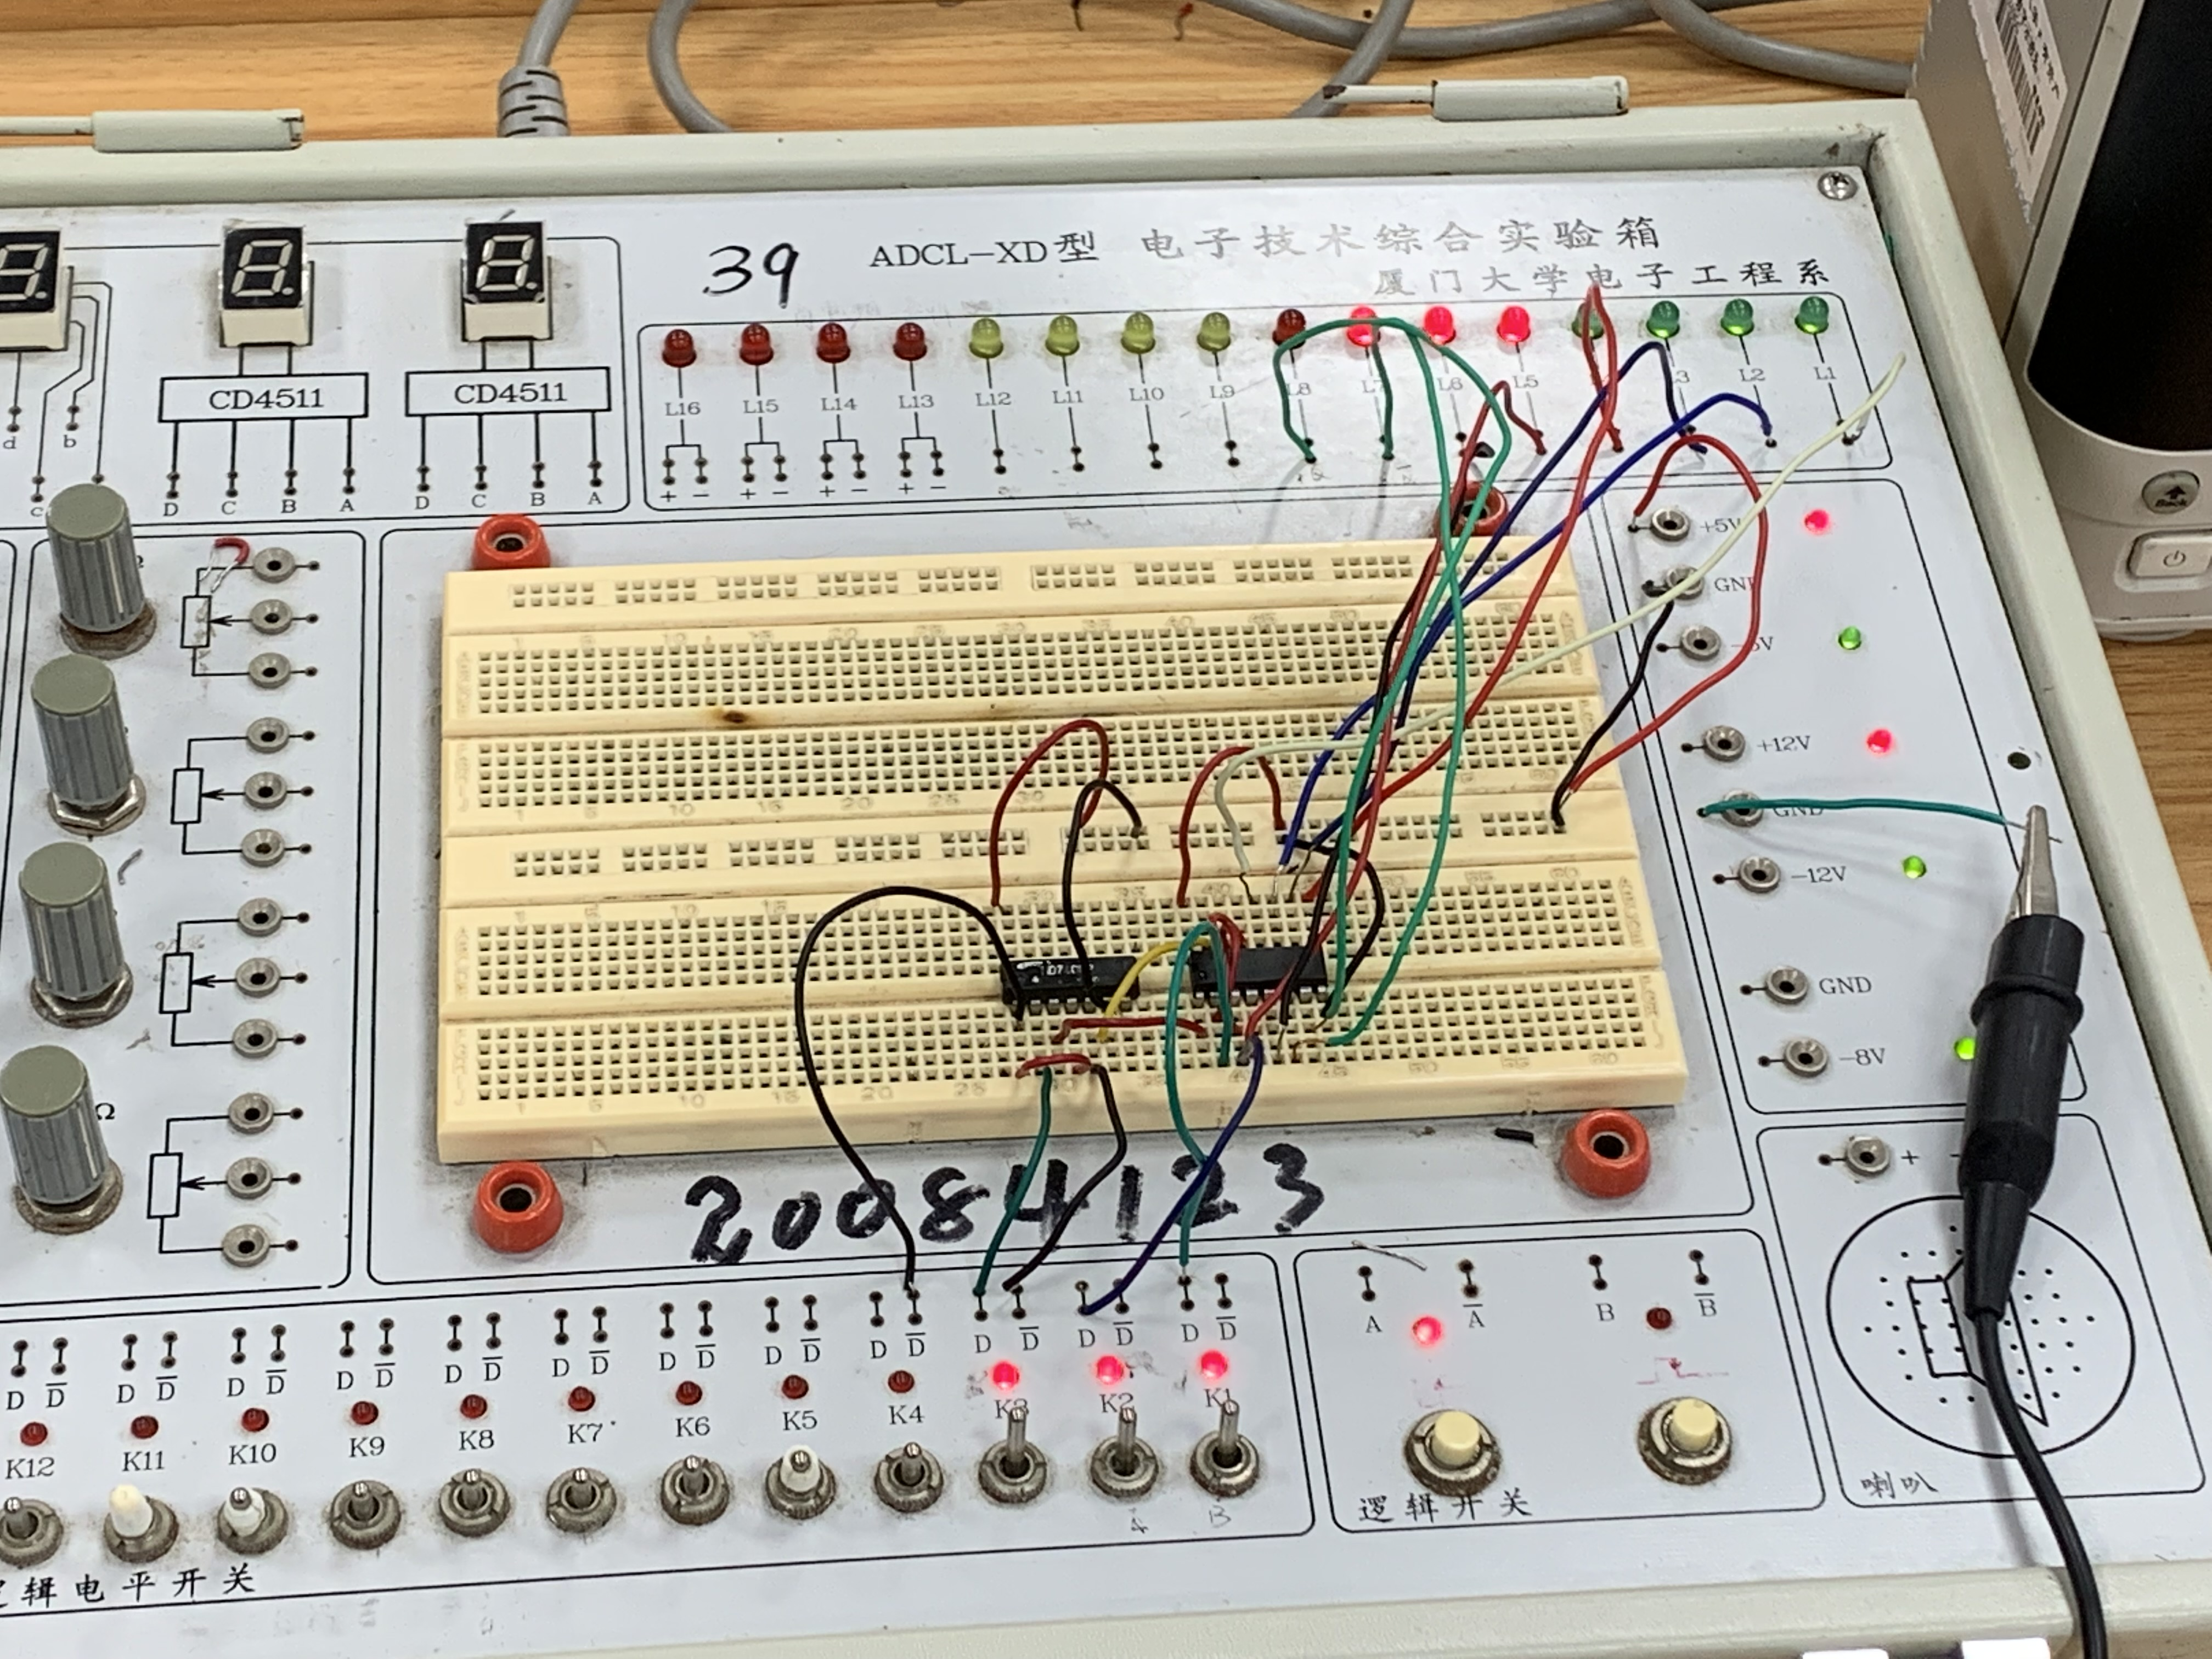
\includegraphics[width=0.48\textwidth]{images/42.JPG}
\end{figure}


填写真值表,得到表~\ref{tbl:resfulladder1},可见实验结果是正确的。

\begin{table}[htbp]
	\centering
	\caption{全加器}
	\label{tbl:resfulladder1}
	\begin{tabular}{ccc|cc}
		\toprule
		\hline
		$A_i$&$B_i$&$C_{i-1}$&$S_i$&$C_i$\\
		\hline
		0&0&0&0&0\\
		0&0&1&1&0\\
		0&1&0&1&0\\
		0&1&1&0&1\\
		1&0&0&1&0\\
		1&0&1&0&1\\
		1&1&0&0&1\\
		1&1&1&1&1\\
		\hline
		\bottomrule
	\end{tabular}
\end{table}

\subsection{多路选择器实现全加器}

按照图连接电路,填写真值表,得到表~\ref{tbl:resfulladder2},可见实验结果是正确的。

\begin{table}[htbp]
	\centering
	\caption{全加器}
	\label{tbl:resfulladder2}
	\begin{tabular}{ccc|cc}
		\toprule
		\hline
		$A_i$&$B_i$&$C_{i-1}$&$S_i$&$C_i$\\
		\hline
		0&0&0&0&0\\
		0&0&1&1&0\\
		0&1&0&1&0\\
		0&1&1&0&1\\
		1&0&0&1&0\\
		1&0&1&0&1\\
		1&1&0&0&1\\
		1&1&1&1&1\\
		\hline
		\bottomrule
	\end{tabular}
\end{table}

\end{spacing}

\end{document}